\documentclass[conference,a4paper]{IEEEtran}
\usepackage[T1]{fontenc}
\usepackage[utf8]{inputenc}
\usepackage{graphicx}
\graphicspath{{screenshots/}}
\usepackage{booktabs}
\usepackage{tabularx}
\usepackage{array}
\usepackage{multirow}
\usepackage{amsmath}
\usepackage{url}
\usepackage{hyperref}
\usepackage{xcolor}
\usepackage{tikz}
\usepackage{listings}
\usetikzlibrary{arrows.meta,positioning,shapes.geometric,fit,calc,backgrounds}
\hypersetup{colorlinks=true,linkcolor=blue!40!black,urlcolor=blue!50!black,citecolor=blue!40!black,pdftitle={AI-Powered Smart Farming},pdfauthor={Manthan Kuvadiya and Kunj Lunagariya}}
\renewcommand{\arraystretch}{1.08}
\definecolor{sfblue}{RGB}{31,78,121}
\definecolor{sfgreen}{RGB}{53,112,75}
\definecolor{sfgray}{RGB}{245,247,250}
\definecolor{sfamber}{RGB}{183,113,23}
\tikzset{
  block/.style={rectangle, rounded corners, draw=sfblue, thick, fill=blue!5,text width=3.0cm, minimum height=0.95cm, align=center},
  smallblock/.style={rectangle, rounded corners, draw=sfgreen, thick, fill=green!5,text width=2.45cm, minimum height=0.8cm, align=center},
  decision/.style={diamond, draw=sfamber, thick, fill=orange!8,aspect=2, text width=2.1cm, align=center, inner sep=2pt},
  datastore/.style={cylinder, shape border rotate=90, aspect=0.25, draw=gray!70,fill=gray!8, thick, minimum height=1.0cm, minimum width=2.2cm, align=center},
  line/.style={-{Stealth[length=2mm]}, semithick, draw=gray!75},
  layer/.style={draw=gray!65, rounded corners=2pt, fill=gray!3, inner sep=7pt},
  stage/.style={rectangle, draw=sfblue!85, fill=blue!3, rounded corners=2pt, line width=0.6pt, text width=2.05cm, minimum height=0.9cm, align=center, font=\scriptsize},
  infra/.style={rectangle, draw=sfgreen!85, fill=green!3, rounded corners=2pt, line width=0.6pt, text width=2.05cm, minimum height=0.85cm, align=center, font=\scriptsize},
  note/.style={font=\scriptsize, text=gray!80!black, align=center},
  flowarrow/.style={-{Stealth[length=1.8mm]}, draw=gray!75, line width=0.6pt},
  decisionbox/.style={rectangle, draw=sfamber, fill=orange!5, rounded corners=2pt, line width=0.7pt, text width=2.0cm, minimum height=0.75cm, align=center, font=\scriptsize}
}
\begin{document}
\title{AI-Powered Smart Farming: Crop Identification, Disease Diagnosis, and Context-Aware Advisory\thanks{Source code repository: \url{https://github.com/manthan2876/Smart-Farming}. Live production deployment: \url{https://smart-farming-dashboard-green.vercel.app}.}}
\author{\IEEEauthorblockN{Manthan Kuvadiya\IEEEauthorrefmark{1} and Kunj Lunagariya\IEEEauthorrefmark{2}}%
\IEEEauthorblockA{Department of Information Technology, CSPIT, CHARUSAT\\
Changa, Gujarat, India\\
Email: \IEEEauthorrefmark{1}23it050@charusat.edu.in, \IEEEauthorrefmark{2}23it053@charusat.edu.in\\
Project Guide: Prof. Rajnik Katariya \quad | \quad Academic Year 2026--2027}}
\maketitle
\begin{abstract}
AI-Powered Smart Farming is an end-to-end, production-grade foliar disease diagnostic and agronomic intelligence platform architected for Indian agriculture. A farmer submits a crop leaf photograph via web or mobile client; within seconds, the system verifies foliage quality, identifies the crop species, classifies the specific pathology, estimates lesion severity, detects insect vectors, ingests live ambient weather, and synthesizes grounded agronomic recommendations in regional vernaculars (English, Hindi, Gujarati) complete with neural audio narration. The platform targets five primary regional crop varieties: Cotton, Groundnut, Pepper Bell, Potato, and Tomato across 32 foliar conditions.

The vision stack is architected as an ensemble: OpenCV HSV segmentation for fail-fast foliage quality gating, EfficientNet-B0 for five-way crop identification, dedicated crop-specific EfficientNet-B2 neural classifiers for pathology diagnosis, adaptive HSV color segmentation for quantitative lesion severity estimation (Healthy, Low $<$15\%, Medium 15--40\%, High $>$40\%), and an Ultralytics YOLOv8-nano classification model for selected insect pests (Aphid, Army Worm, Leaf Miner, Spider Mite). Agronomic guidance is grounded in an ICAR/KVK-aligned knowledge base (56 condition entries, 155 aliases) paired with Groq Llama-3.3-70B and TF-IDF RAG safety guardrails enforcing banned agrochemical exclusion. Vernacular translation uses a zero-hang multi-tiered IndicTrans2 engine with a 400+ domain lexicon cache, while speech playback is synthesized via Microsoft Edge-TTS with on-device mobile fallback. The infrastructure decouples a React 19/Vite web application (Vercel) and Flutter mobile client from a FastAPI API gateway (Render) and a consolidated AI microservice on Hugging Face Spaces (port 7860). Supabase provides managed PostgreSQL and private object storage with 15-minute signed URLs; Upstash supplies Redis REST dedup caching (24-hour TTL, $<$20\,ms repeat turnaround) and QStash scheduled crons for proactive weather alerts. Security incorporates Argon2id password hashing, database-backed refresh token rotation with token family reuse compromise detection, 1-tap guest sessions, and Supabase Remote Config backend URL locking. MLOps continuous retraining enforces a zero-leakage spatial deterministic split hashed on \texttt{plot\_id}, 70/30 replay buffer mixing to prevent catastrophic forgetting, and atomic model registry promotion.
\end{abstract}
\begin{IEEEkeywords}
Smart agriculture, crop identification, plant disease classification, EfficientNet, YOLOv8, FastAPI, multilingual advisory, MLOps, expert review, free-tier deployment.
\end{IEEEkeywords}


% ---------------- Section ----------------
\section{Introduction}
\subsection{Background}
Agriculture is affected by crop disease, pests, changing weather, nutrient deficiencies, and differences between controlled and field conditions. Timely recognition of visible symptoms can help a farmer decide whether to inspect a crop more closely, seek expert advice, or take a suitable next step. Manual diagnosis remains valuable, but it may be limited by access to experts, language barriers, and the time required to inspect many plants.

Computer vision can classify visual patterns in crop images, while a backend platform can connect those predictions to farmer history, plot information, weather observations, and structured recommendations. A practical system must do more than return a class label: it should validate the uploaded image, communicate uncertainty, preserve the history of decisions, protect user data, and support correction when an automated result is questionable.

\subsection{Project overview}
The AI-Powered Smart Farming project is an end-to-end software platform for crop-leaf diagnosis and agricultural decision support engineered specifically for Indian regional agriculture. Its crop identifier covers Cotton, Groundnut, Pepper Bell, Potato, and Tomato. Dedicated per-crop neural classifiers follow crop identification across 32 pathologically verified conditions, while subsequent pipeline stages quantify visible infection severity via adaptive HSV color segmentation, classify selected insect pest vectors via Ultralytics YOLOv8-nano, retrieve live meteorological observations via OpenWeatherMap, and generate an agronomist-validated, ICAR/KVK-grounded four-field advisory. User interactions are supported through a responsive React 19/TypeScript web client deployed globally on Vercel at \url{https://smart-farming-dashboard-green.vercel.app} and a Flutter mobile client incorporating keyless Leaflet GIS boundary mapping and trilingual neural speech narration (English, Hindi, Gujarati). Administrative workflows provide agronomist triage review, automated drift monitoring, and a zero-leakage continuous retraining pipeline. The complete open-source codebase, ML artifacts, and deployment orchestration are publicly maintained on GitHub at \url{https://github.com/manthan2876/Smart-Farming}.

\subsection{Problem statement}
Smallholder farmers frequently encounter crop yield devastation from foliar fungal, bacterial, and viral pathogens due to delayed diagnosis, lack of local agricultural extension officers, and literacy or language barriers. While automated computer-vision classifiers exist, practical deployment requires bridging visual inference with real-world farm context, transparent confidence escalation, regional language accessibility, and strict safety guardrails against off-label chemical pesticide misuse. A dependable platform must reject poor-quality or non-foliar uploads, distinguish unsupported species, preserve immutable provenance, provide human-in-the-loop expert review for ambiguous predictions, and maintain a rigorous MLOps lifecycle to prevent dataset leakage during retraining.

\subsection{Objectives}
\begin{enumerate}
  \item Perform fast-fail image validation using OpenCV Laplacian variance, luminance thresholds, and HSV vegetation isolation.
  \item Identify the crop species across five primary regional varieties (Cotton, Groundnut, Pepper Bell, Potato, Tomato) using EfficientNet-B0 with post-hoc temperature calibration.
  \item Route validated foliage images to dedicated per-crop EfficientNet-B2 neural classifiers across 32 foliar conditions.
  \item Estimate quantitative lesion coverage via adaptive HSV color segmentation into standardized severity buckets (Healthy, Low, Medium, High) with false-contour suppression on healthy leaves.
  \item Classify supported insect pest vectors (Aphid, Army Worm, Leaf Miner, Spider Mite) using an Ultralytics YOLOv8-nano model with explicit tri-state availability reporting.
  \item Synthesize structured four-field agronomic guidance (Immediate Action, Chemical/Bio Treatment, Cultural Prevention, Monitoring) grounded in ICAR/KVK schedules with RAG banned-chemical exclusion.
  \item Provide complete trilingual regional accessibility (English, Hindi, Gujarati) powered by a zero-hang multi-tiered IndicTrans2 engine and Microsoft Edge-TTS neural speech narration.
  \item Support keyless GIS field boundary mapping via Leaflet (OSM/Satellite) with geodesic acreage calculations and Shapely self-intersection validation.
  \item Maintain prediction provenance, longitudinal rescan tracking, Upstash Redis REST dedup caching, and proactive QStash weather-risk crons.
  \item Support human-in-the-loop agronomist triage with atomic review claiming, override prescription, and automated farmer alert dispatch.
  \item Implement a zero-leakage MLOps export pipeline using spatial deterministic hashing on \texttt{plot\_id}, 70/30 replay buffer mixing, and atomic model registry promotion with rollback.
  \item Operate within resilient, low-cost serverless hosting constraints (Vercel, Render, Hugging Face Spaces, Supabase, Upstash) with automated keepalive orchestration.
\end{enumerate}

\subsection{Scope and boundaries}
The documented implementation is an image-based decision-support platform. It is not a substitute for a qualified agronomist, laboratory diagnosis, or local pesticide-label guidance. The system only supports its configured crop and disease classes. It should not claim a definitive diagnosis for an unknown crop, an image outside the training distribution, or a low-confidence result. Weather and farm-context features improve context but do not, by themselves, prove the cause of a plant symptom.

Report organisation: The paper is organised as follows. Section II presents motivation and requirements; Section III describes the architecture; Sections IV and V discuss data and the inference pipeline; subsequent sections cover APIs, security, MLOps, evaluation, deployment, limitations, future work, and conclusions.
% ---------------- Section ----------------
\section{Existing System, Motivation and Requirements}
\subsection{Motivation}
A useful agricultural AI application must bridge several distinct tasks: vision inference, agronomic interpretation, regional-language communication, and ongoing record management. A standalone image classifier solves only part of the problem. Smart Farming connects prediction outputs with farm and plot records, historical scans, weather context, multilingual content, and human review.

\subsection{Existing workflow challenges}
Common challenges in a manual or fragmented workflow include delayed access to expert guidance, inconsistent descriptions of symptoms, difficulty comparing the same plant over time, and limited traceability of the recommendation that was shown to a farmer. A computer-vision model can also fail when a field image differs from its training data. The project therefore includes image validation, confidence-aware review, historical records, and a route for experts to correct or override a result.

\subsection{Functional requirements}
\begin{table*}[!t]
\centering
\small
\caption{Functional Requirements and Implementation Status}
\label{tab:functional_requirements}
\begin{tabularx}{\textwidth}{l p{3.8cm} X}
\toprule
\textbf{ID} & \textbf{Requirement} & \textbf{Implemented behaviour}\\
\midrule
FR-01 & Account management & Register and authenticate users via email or phone/OTP; Argon2id password hashing via \texttt{pwdlib}; database-backed refresh token rotation with token family reuse compromise detection; 1-tap ephemeral guest mode (\texttt{/api/v1/auth/guest}).\\
FR-02 & Image submission & Accept JPEG, PNG, or WebP leaf uploads up to 10 MB; binary magic-byte decoding via PIL \texttt{Image.verify()}; compute SHA-256 content hash; store in Supabase Object Storage with 15-minute signed URLs.\\
FR-03 & Image validation & Check Upstash Redis REST dedup cache (\texttt{sf:dedup:\{hash\}}, 24\,h TTL, $<$20\,ms repeat response); OpenCV Laplacian-variance blur ($>50$), luminance bounds (40--240), and HSV foliage segmentation with structured error messages.\\
FR-04 & Crop identification & EfficientNet-B0 five-way classifier (Cotton, Groundnut, Pepper Bell, Potato, Tomato); calibrated with post-hoc temperature scaling ($T=1.08$, ECE 0.0072); provenance block records model version and latency.\\
FR-05 & Disease classification & Route to dedicated crop-specific EfficientNet-B2 neural classifiers covering 32 verified conditions; logit scaling ($T \in [1.10, 1.18]$); uncertainty cutoff ($<0.70$) triggers automatic agronomist escalation.\\
FR-06 & Severity estimation & Adaptive HSV color segmentation computes visible lesion area percentage into standardized buckets: Healthy (0\%), Low ($<$15\%), Medium (15--40\%), and High ($>$40\%); false-contour suppression on healthy leaves; JET Grad-CAM generation.\\
FR-07 & Pest classification & Ultralytics YOLOv8-nano classification across supported insect vectors (Aphid, Army Worm, Leaf Miner, Spider Mite); tri-state status reporting (\texttt{no\_pests\_detected}, \texttt{pest\_detected}, \texttt{unavailable}).\\
FR-08 & Contextual advisory & Four-field output (Immediate Action, Chemical/Bio Treatment, Cultural Prevention, Monitoring); grounded in deterministic ICAR/KVK KB v2 (56 conditions, 155 aliases, 0\,ms CPU latency) paired with Groq Llama-3.3-70B and TF-IDF RAG banned-chemical exclusion.\\
FR-09 & Localisation \& TTS & Trilingual support (English, Hindi, Gujarati) powered by multi-tiered zero-hang IndicTrans2 engine (400+ domain cache, sentence chunking, greedy Seq2Seq); neural speech narration via Microsoft Edge-TTS with mobile on-device fallback.\\
FR-10 & History and rescan & Longitudinal diagnostic archive; rescan linking connects follow-up leaf captures to earlier scans to evaluate symptom progression over time.\\
FR-11 & Expert review & Agronomist review desk (\texttt{/admin/expert}) with atomic claim locks, decision recording (Approve, Override, Request Rescan), verified alert dispatch, and retraining candidate flagging.\\
FR-12 & Feedback collection & In-situ farmer accuracy feedback (correct/incorrect) and optional notes logged for model drift telemetry and agronomist inspection.\\
FR-13 & GIS Farm and plots & Keyless Leaflet mapping (OSM / Esri Satellite) with geodesic acreage calculation; Shapely self-intersection validation; ray-casting plot-in-farm containment (\texttt{\_plot\_inside\_farm}); mobile magnetic snapping.\\
FR-14 & Alerts and weather & Live OpenWeatherMap data cached in Upstash Redis REST (10--30\,min TTL); scheduled QStash cron webhooks (\texttt{/internal/cron/weather-risks}) generate proactive alerts for rainfall ($>$20\,mm) and high fungal sporulation risk.\\
FR-15 & MLOps lifecycle & Zero-leakage spatial deterministic dataset export hashed on \texttt{plot\_id}; 70/15/15 train/val/test split; 70/30 replay buffer mixing; automatic EXIF coordinate scrubbing; atomic model registry promotion and version rollback.\\
\bottomrule
\end{tabularx}
\end{table*}

\subsection{Non-functional requirements}
\begin{table*}[!t]
\centering
\small
\caption{Non-Functional Requirements and System Quality Attributes}
\label{tab:non_functional_requirements}
\begin{tabularx}{\textwidth}{p{3.2cm} X}
\toprule
\textbf{Category} & \textbf{Requirement}\\
\midrule
Security & JWT authentication, role-based authorisation, password hashing, secure refresh cookies, rate limiting, and scoped media access.\\
Reliability & Clear pipeline-stage status, controlled failure responses, and a fallback or escalation path for uncertain predictions.\\
Maintainability & Configuration-driven thresholds, separable AI service, versioned model artefacts, and documented API contracts.\\
Performance & Avoid unnecessary model loading and expensive inference; use caching for appropriate repeat requests.\\
Usability & Farmer-oriented workflows, clear explanations, accessible language, and concise next actions.\\
Localisation & Support the user's preferred language and regional-language narration.\\
Auditability & Preserve prediction provenance, model versions, expert corrections, and training/export metadata.\\
Cost & Prefer free-tier or low-cost services, while documenting sleep, CPU, memory, quota, and cold-start constraints.\\
\bottomrule
\end{tabularx}
\end{table*}

\subsection{Users and roles}
The documented platform has three roles. Farmers use diagnosis, history, farm records, alerts, feedback, and expert escalation. Experts inherit farmer permissions and can review queued cases, inspect associated media, submit review decisions, and flag appropriate cases for retraining. Administrators inherit expert permissions and additionally manage users, configuration, platform metrics, model operations, and maintenance tasks. Elevated roles are assigned by an administrator rather than selected freely at ordinary registration.

% ---------------- Section ----------------
\section{System Architecture}
\subsection{Architecture overview}
The platform separates public-facing API orchestration from compute-intensive neural inference. The web client is deployed globally on Vercel at \url{https://smart-farming-dashboard-green.vercel.app}, with all platform services version-controlled in the official repository at \url{https://github.com/manthan2876/Smart-Farming}. The API gateway on Render is built with FastAPI \cite{ref8} and handles authentication, multipart validation, image hashing, Upstash Redis REST dedup caching, PostgreSQL persistence, signed media URL issuance, and workflow scheduling. The unified AI microservice on Hugging Face Spaces \cite{ref10} (\texttt{Maharsh8805/smart-farming-ai}, port 7860) hosts the seven-stage vision ensemble, IndicTrans2 translation, and Edge-TTS synthesis. Managed PostgreSQL on Supabase \cite{ref11} stores relational entities and full prediction provenance; Supabase Object Storage isolates original and processed media behind time-bounded signed URLs (15-minute expiry); Upstash Redis REST provides in-memory dedup and weather caching; and QStash triggers scheduled cron webhooks.

\begin{figure*}[!t]
\centering
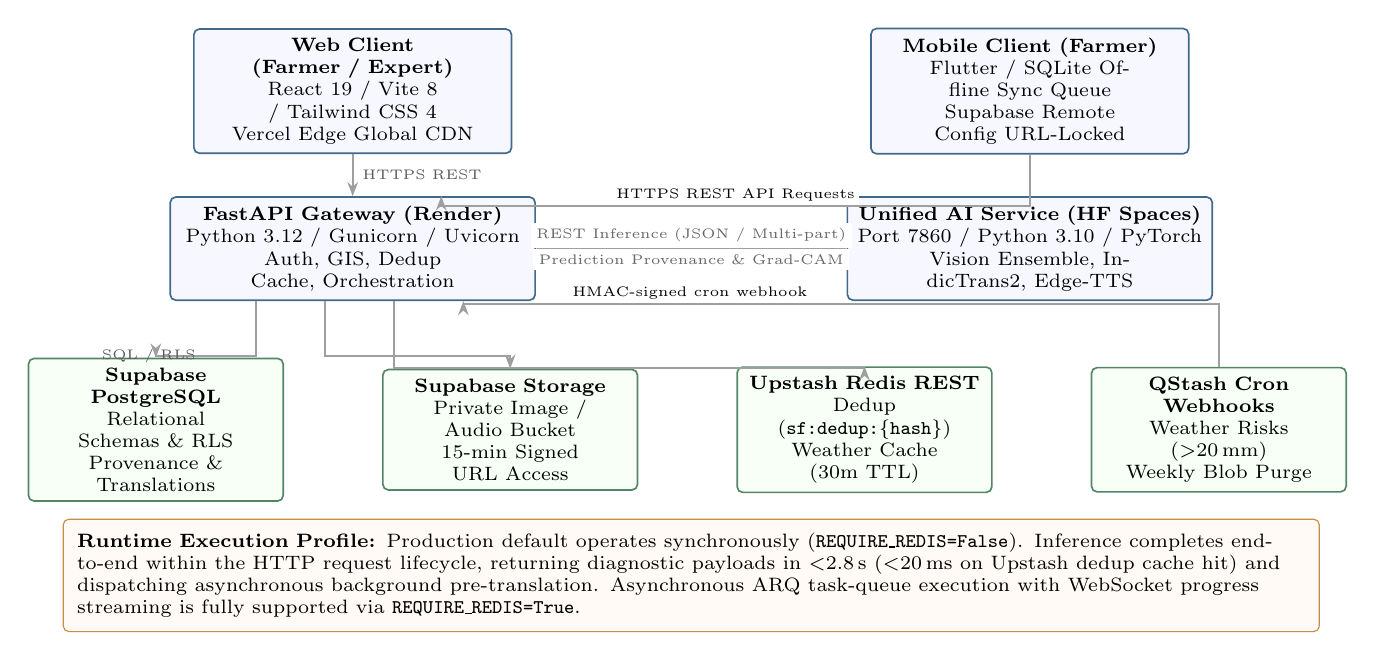
\begin{tikzpicture}[x=1cm,y=1cm]
% Tier 1: Client Interfaces
\node[stage,text width=3.8cm,minimum height=1.05cm] (web) at (4.3, 3.8) {%
  \textbf{Web Client (Farmer / Expert)}\\
  React 19 / Vite 8 / Tailwind CSS 4\\
  Vercel Edge Global CDN};

\node[stage,text width=3.8cm,minimum height=1.05cm] (mobile) at (12.9, 3.8) {%
  \textbf{Mobile Client (Farmer)}\\
  Flutter / SQLite Offline Sync Queue\\
  Supabase Remote Config URL-Locked};

% Tier 2: Core Application & Inference Services
\node[stage,text width=4.4cm,minimum height=1.2cm] (api) at (4.3, 1.8) {%
  \textbf{FastAPI Gateway (Render)}\\
  Python 3.12 / Gunicorn / Uvicorn\\
  Auth, GIS, Dedup Cache, Orchestration};

\node[stage,text width=4.4cm,minimum height=1.2cm] (ai) at (12.9, 1.8) {%
  \textbf{Unified AI Service (HF Spaces)}\\
  Port 7860 / Python 3.10 / PyTorch\\
  Vision Ensemble, IndicTrans2, Edge-TTS};

% Tier 3: Persistence & External Infrastructure
\node[infra,text width=3.0cm,minimum height=1.05cm] (db) at (1.8, -0.5) {%
  \textbf{Supabase PostgreSQL}\\
  Relational Schemas \& RLS\\
  Provenance \& Translations};

\node[infra,text width=3.0cm,minimum height=1.05cm] (obj) at (6.3, -0.5) {%
  \textbf{Supabase Storage}\\
  Private Image / Audio Bucket\\
  15-min Signed URL Access};

\node[infra,text width=3.0cm,minimum height=1.05cm] (cache) at (10.8, -0.5) {%
  \textbf{Upstash Redis REST}\\
  Dedup (\texttt{sf:dedup:\{hash\}})\\
  Weather Cache (30m TTL)};

\node[infra,text width=3.0cm,minimum height=1.05cm] (jobs) at (15.3, -0.5) {%
  \textbf{QStash Cron Webhooks}\\
  Weather Risks ($>$20\,mm)\\
  Weekly Blob Purge};

% Inter-tier Connections
% Client -> Gateway
\draw[flowarrow] (web.south) -- node[right,font=\tiny,text=gray!70!black]{HTTPS REST} (api.north);
\draw[flowarrow] (mobile.south) -- ++(0,-0.65) -| node[pos=0.25,above,font=\tiny,fill=white,inner sep=1.5pt]{HTTPS REST API Requests} ([xshift=32pt]api.north);

% Gateway <-> AI Service
\draw[{Stealth[length=1.8mm]}-{Stealth[length=1.8mm]}, draw=gray!75, line width=0.6pt] (api.east) -- 
  node[above,font=\tiny,text=gray!80!black,fill=white,inner sep=2pt]{REST Inference (JSON / Multi-part)} 
  node[below,font=\tiny,text=gray!80!black,fill=white,inner sep=2pt]{Prediction Provenance \& Grad-CAM} (ai.west);

% Gateway -> Storage & Persistence
\draw[flowarrow] ([xshift=-35pt]api.south) -- ++(0,-0.7) -| node[pos=0.25,left,font=\tiny,text=gray!70!black]{SQL / RLS} (db.north);
\draw[flowarrow] ([xshift=-10pt]api.south) -- ++(0,-0.7) -| (obj.north);
\draw[flowarrow] ([xshift=15pt]api.south) -- ++(0,-0.85) -| (cache.north);

% QStash Webhooks -> Gateway (Orthogonal corridor routing)
\draw[flowarrow] (jobs.north) -- ++(0,0.8) -| node[pos=0.35,above,font=\tiny,fill=white,inner sep=1.5pt]{HMAC-signed cron webhook} ([xshift=40pt]api.south);

% Callout Box: Runtime Execution Profile
\node[draw=sfamber!80,fill=orange!4,rounded corners=2pt,text width=15.6cm,align=left,inner sep=5pt,font=\scriptsize] at (8.6,-2.35) {%
  \textbf{Runtime Execution Profile:} Production default operates synchronously (\texttt{REQUIRE\_REDIS=False}). Inference completes end-to-end within the HTTP request lifecycle, returning diagnostic payloads in $<$2.8\,s ($<$20\,ms on Upstash dedup cache hit) and dispatching asynchronous background pre-translation. Asynchronous ARQ task-queue execution with WebSocket progress streaming is fully supported via \texttt{REQUIRE\_REDIS=True}.%
};
\end{tikzpicture}
\caption{Deployment-oriented logical architecture illustrating decoupled microservices, storage boundaries, and scheduled cron integrations.}
\label{fig:architecture}
\end{figure*}

\subsection{Application layers}
\textbf{Client layer:} The web application is built with React 19, TypeScript, Vite 8, and Tailwind CSS 4, deployed on Vercel Edge. It integrates an interactive Leaflet GIS map with satellite overlays for field polygon drafting, Lucide React icons, and trilingual UI catalogs. The Flutter mobile app operates a phone-first farmer persona with five-tab navigation (\texttt{FarmerShell}), an offline SQLite scan queue (\texttt{SyncService}), on-device 1024px photo compression, and strict backend URL locking via Supabase Remote Config.

\textbf{API gateway:} The FastAPI service on Render acts as the secure entrypoint. It validates file magic bytes via PIL, checks the Upstash Redis REST dedup cache, enforces Argon2id password authentication, rotates database-backed refresh tokens, computes geodesic field acreage, and stores prediction provenance.

\textbf{AI inference layer:} The unified AI microservice is deployed on a dedicated Hugging Face Space (\texttt{Maharsh8805/smart-farming-ai}, port 7860). It encapsulates OpenCV quality analysis, EfficientNet-B0 crop classification, per-crop EfficientNet-B2 disease models, adaptive HSV lesion segmentation, YOLOv8-nano pest classification, IndicTrans2 translation, and Edge-TTS narration behind unified REST endpoints.

\textbf{Data and storage layer:} Supabase PostgreSQL manages relational entities with Row Level Security (RLS). Supabase Object Storage isolates original photos, processed masks, and audio files. Upstash Redis REST provides stateless HTTP-based caching. Scheduled background tasks (proactive weather risks and orphaned blob pruning) are executed via Upstash QStash webhooks verified with cryptographic HMAC signatures.

\subsection{Synchronous and asynchronous modes}
The platform supports dual runtime execution modes configured via \texttt{REQUIRE\_REDIS}:
\begin{itemize}
  \item \textbf{Synchronous cloud mode (\texttt{REQUIRE\_REDIS=False}, production default):} The prediction request runs the complete vision and advisory pipeline synchronously within the HTTP request. Completed findings are saved to the Upstash Redis REST dedup cache (\texttt{sf:dedup:\{hash\}}, 24-hour TTL) and committed to PostgreSQL. A repeat upload of the same leaf returns immediately in under 20\,ms. Concurrently, \texttt{FastAPI.BackgroundTasks} pre-translates the recommendation into Hindi and Gujarati, persisting them into the \texttt{entity\_translations} table for instantaneous client localization.
  \item \textbf{Asynchronous worker mode (\texttt{REQUIRE\_REDIS=True}):} The API enqueues the job into an ARQ worker pool and returns an immediate HTTP 202 status with a prediction identifier. The worker executes each pipeline stage, publishing Redis pub/sub progress events streamed to clients via WebSockets (\texttt{/ws/predictions/\{id\}}).
\end{itemize}

\begin{figure*}[!t]
\centering
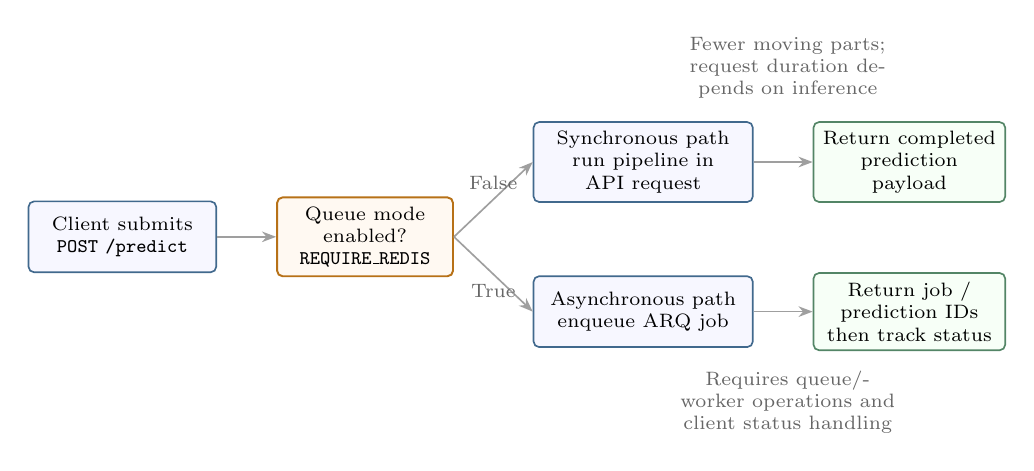
\begin{tikzpicture}[node distance=0.65cm and 0.75cm]
\node[stage, text width=2.15cm] (request) {Client submits\\\texttt{POST /predict}};
\node[decisionbox, right=of request, text width=2.0cm] (mode) {Queue mode enabled?\\\texttt{REQUIRE\_REDIS}};
\node[stage, right=1.0cm of mode, yshift=0.95cm, text width=2.55cm] (sync) {Synchronous path\\run pipeline in API request};
\node[stage, right=1.0cm of mode, yshift=-0.95cm, text width=2.55cm] (async) {Asynchronous path\\enqueue ARQ job};
\node[infra, right=of sync, text width=2.2cm] (result) {Return completed\\prediction payload};
\node[infra, right=of async, text width=2.2cm] (jobid) {Return job / prediction IDs\\then track status};
\draw[flowarrow] (request) -- (mode);
\draw[flowarrow] (mode.east) -- node[above,note]{False} (sync.west);
\draw[flowarrow] (mode.east) -- node[below,note]{True} (async.west);
\draw[flowarrow] (sync) -- (result);
\draw[flowarrow] (async) -- (jobid);
\node[note, text width=3.2cm] at (8.45,2.15) {Fewer moving parts; request duration depends on inference};
\node[note, text width=3.2cm] at (8.45,-2.1) {Requires queue/worker operations and client status handling};
\end{tikzpicture}
\caption{Prediction execution modes. The synchronous mode is the documented production default; queue mode is enabled only when configured.}
\label{fig:execution-modes}
\end{figure*}

\subsection{Data flow}
A user uploads an image with optional location, language, and plot metadata. The API validates the file and checks for duplicate content. It stores the original image, runs or schedules the pipeline, and persists each stage's output and status. The response includes crop, disease, severity, pests, weather context, recommendation, provenance, and any available translations or review metadata. Media is accessed through role-checked endpoints or short-lived signed URLs.

% ---------------- Section ----------------
\section{Dataset and Label Design}
\subsection{Dataset overview}
The supplied project summary reports a dataset of 34,548 images across five crop categories: Cotton, Groundnut, Pepper Bell, Potato, and Tomato. Images include controlled and field/uncontrolled environments. The dataset is organised into disease or condition subfolders, and the project maintains a folder-renaming reference to normalise the source labels.

\begin{table}[!t]
\centering
\caption{Crop classes in the crop-identification stage}
\label{tab:crop_classes}
\begin{tabularx}{\columnwidth}{lX}
\toprule
\textbf{Class index (illustrative)} & \textbf{Crop label}\\
\midrule
0 & Cotton\\
1 & Groundnut\\
2 & Pepper Bell\\
3 & Potato\\
4 & Tomato\\
\bottomrule
\end{tabularx}
\end{table}
The index-to-label order used by a trained checkpoint must come from its matching label map, not from this illustrative table. Training and inference must use the same mapping.

\begin{figure}[!t]
\centering
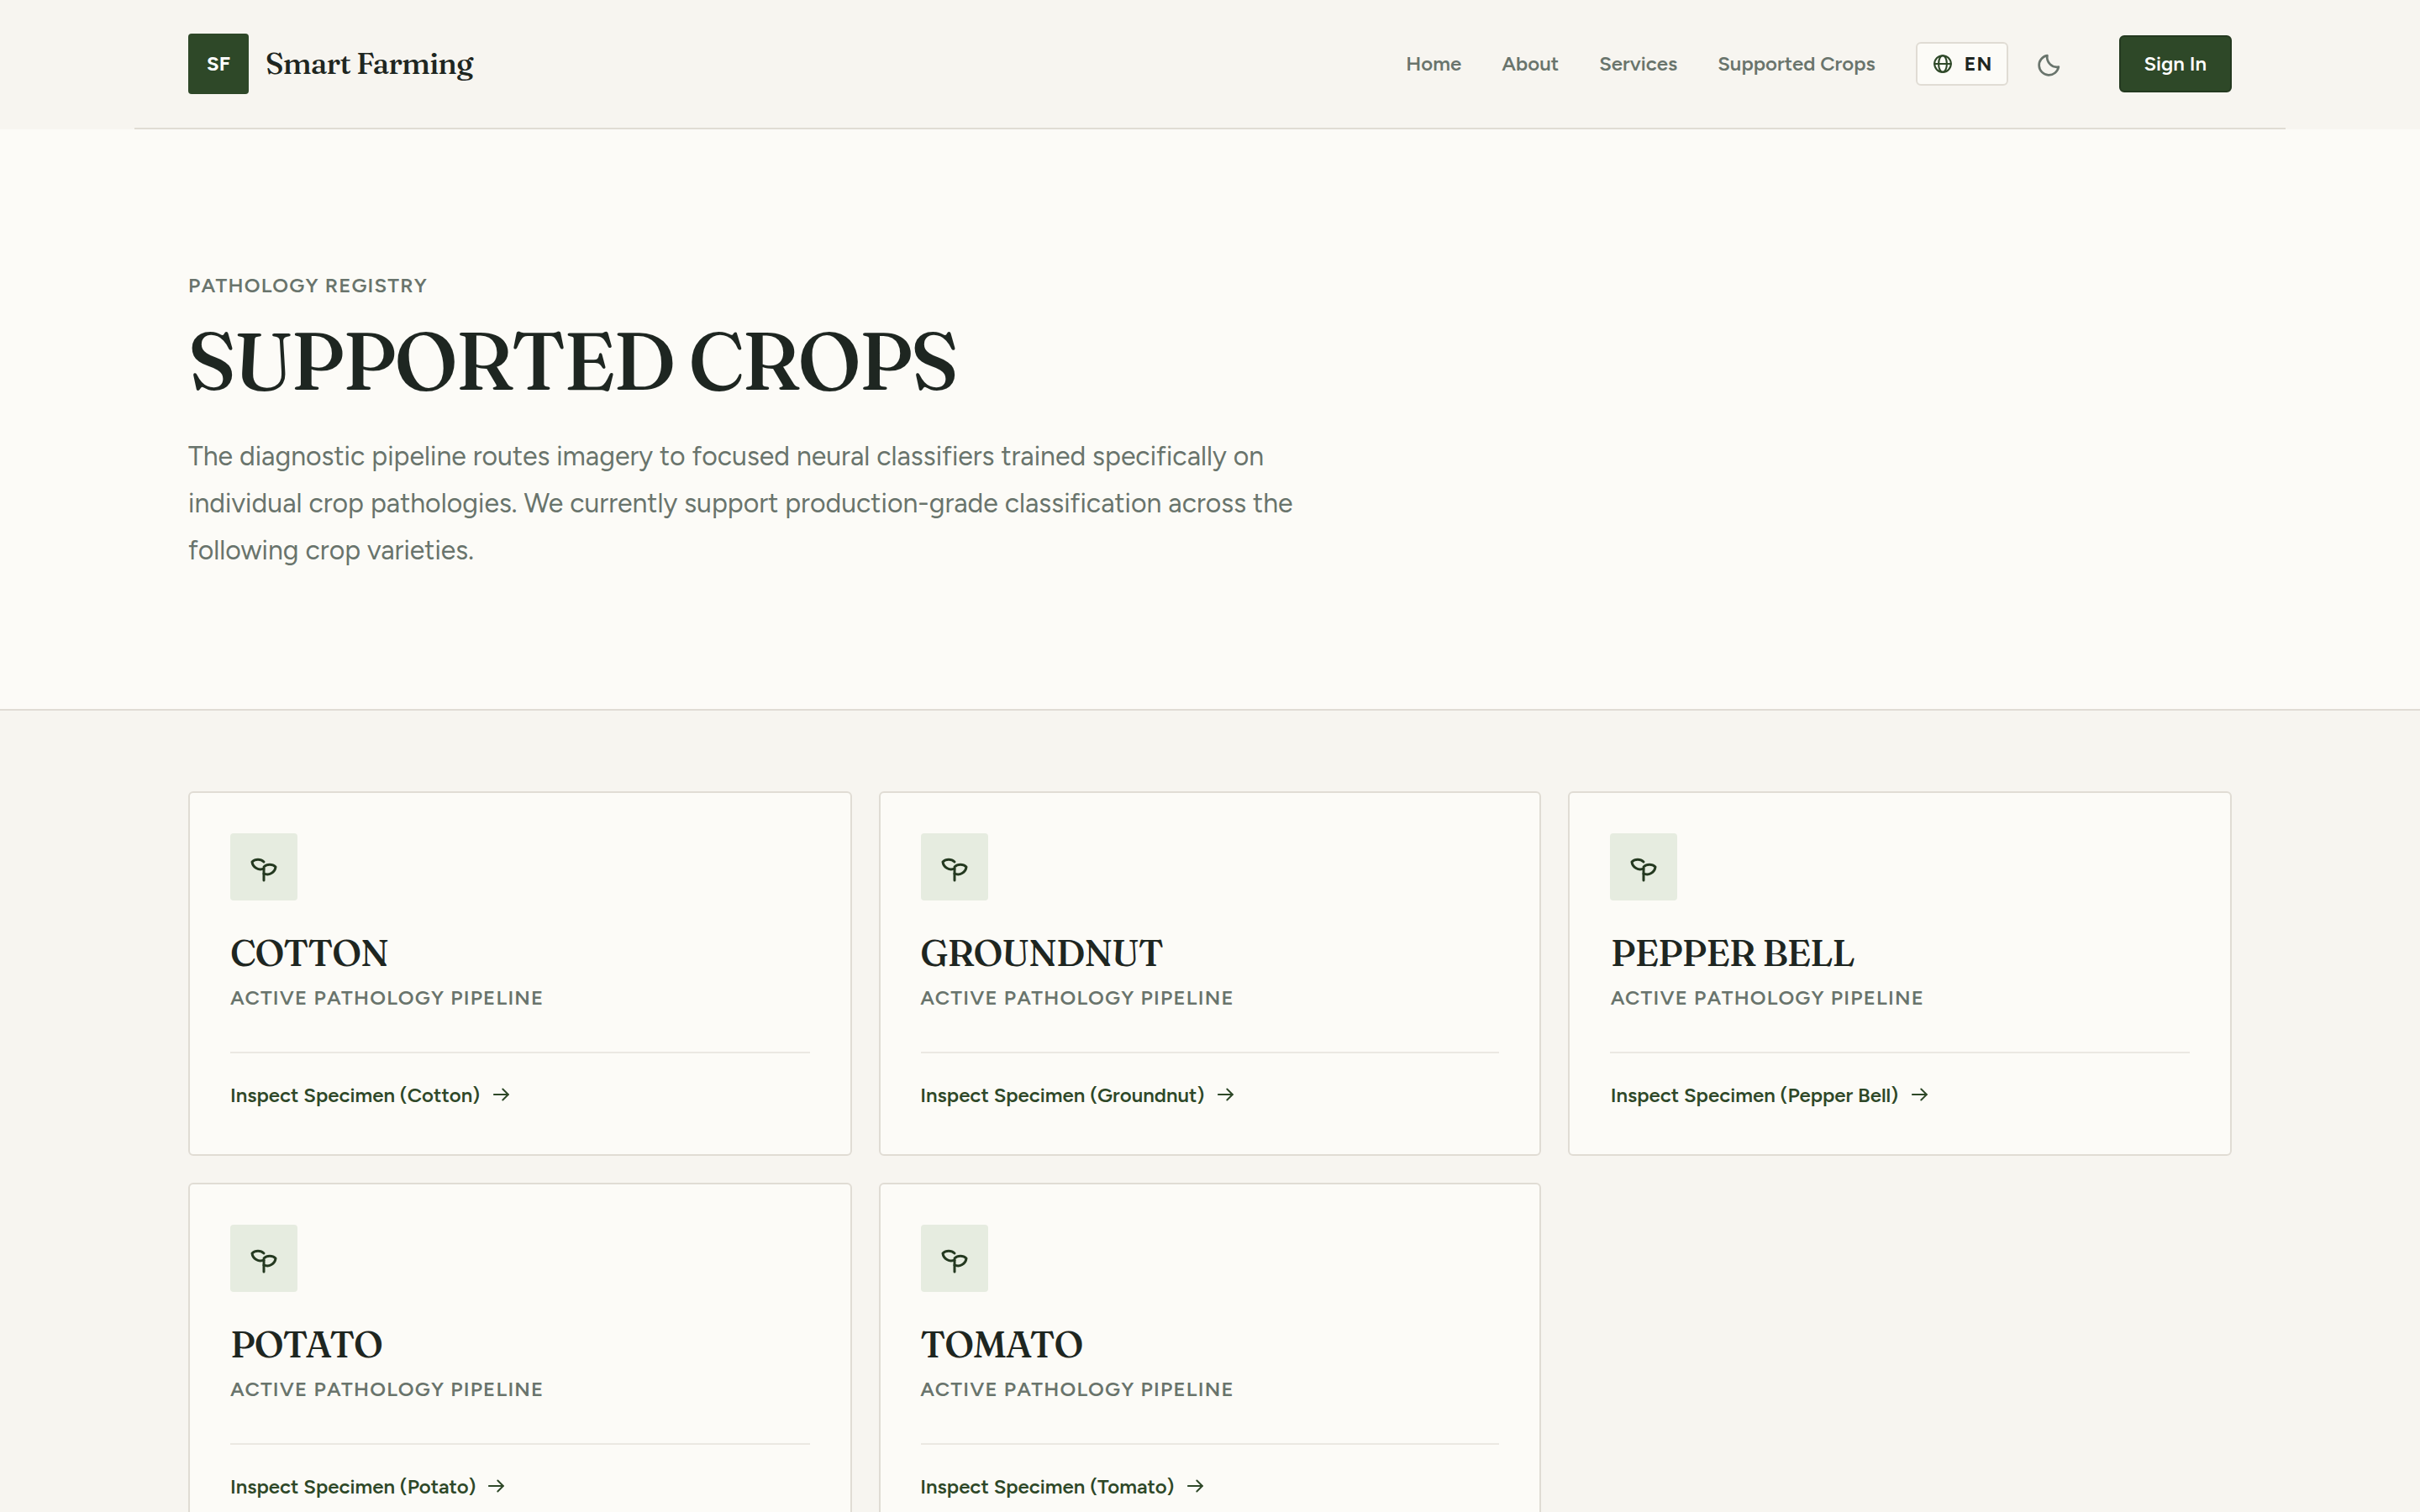
\includegraphics[width=\columnwidth]{screenshots/02_crops_catalog.png}
\caption{Supported crop pathology registry on the platform interface, displaying dedicated classifier routing for Cotton, Groundnut, Pepper Bell, Potato, and Tomato.}
\label{fig:crops-catalog}
\end{figure}

\subsection{Environment variation}
The dataset distinguishes controlled-environment images from uncontrolled or field-captured images. This distinction matters because background clutter, lighting, leaf orientation, multiple leaves, and camera quality can alter the visual distribution. A high score on controlled images alone would not establish field readiness. The newer Model Cards \cite{ref12} report 99.65\% crop-identification accuracy on the controlled subset and 99.35\% on the uncontrolled field subset. The older notebook summary contains different environment figures; this paper uses the newer Model Cards as requested and treats both sets as project-reported rather than independently verified results.

\subsection{Folder-label normalisation}
The supplied folder-renaming reference \cite{ref4} maps original directory names to shorter codes. These codes are useful for file organisation, but they should not become user-facing diagnosis labels. Label normalisation should preserve the original source label and the canonical label in metadata so that data lineage is recoverable. For merged sources, the data manifest should record source dataset, source URL or identifier, original class, canonical class, environment, split, and any expert correction.

\subsection{Data quality and governance}
A reliable training dataset needs checks for corrupt files, exact duplicates, near-duplicates, label conflicts, class imbalance, and distribution leakage. Multiple photos of the same plant or plot should not be randomly scattered across training and test splits if the objective is to estimate performance on unseen plants or plots. The updated MLOps guide \cite{ref3} describes a spatial deterministic split hashed on \texttt{plot\_id} to reduce rescan leakage, a 70/30 replay-buffer mixing strategy, and default use of verified candidates marked \texttt{added\_to\_dataset}. These controls should be verified in the actual export implementation and its metadata.

\subsection{Recommended split policy}
The documented training export example uses 70\% training, 15\% validation, and 15\% test data. The test set should be held out from checkpoint selection and threshold tuning. When data is grouped by plot or plant, group-aware splitting is preferable to simple image-level random splitting. The export should include a manifest and timestamp so that each model result can be linked to the exact data version.

\begin{table}[!t]
\centering
\caption{Dataset governance controls}
\label{tab:governance_controls}
\begin{tabularx}{\columnwidth}{p{3.6cm}X}
\toprule
\textbf{Control} & \textbf{Purpose}\\
\midrule
File integrity check & Reject unreadable or malformed image files.\\
Duplicate detection & Prevent repeated images from inflating metrics or creating repeated submissions.\\
Canonical label map & Ensure class names are consistent across training, evaluation, and inference.\\
Group-aware split & Reduce leakage from repeated scans of the same plot or plant.\\
Expert verification & Prefer reviewed labels for retraining and track correction provenance.\\
Manifest and hashes & Make exports reproducible and auditable.\\
Class-balance report & Detect underrepresented classes before training.\\
\bottomrule
\end{tabularx}
\end{table}

% ---------------- Section ----------------
\section{AI Inference Pipeline}
\subsection{Pipeline stages and architectural orchestration}
The core vision and agronomic inference engine is hosted as a dedicated microservice on Hugging Face Spaces (\texttt{Maharsh8805/smart-farming-ai}, port 7860), decoupled from the Render API gateway. The pipeline executes a 7-stage vision and language ensemble coordinated through a shared context dictionary, where each stage reports granular latency, status codes, and model provenance. This prevents partial failures in optional components (such as pest classification or weather feeds) from silently compromising or discarding primary disease diagnoses.

\begin{figure*}[!t]
\centering
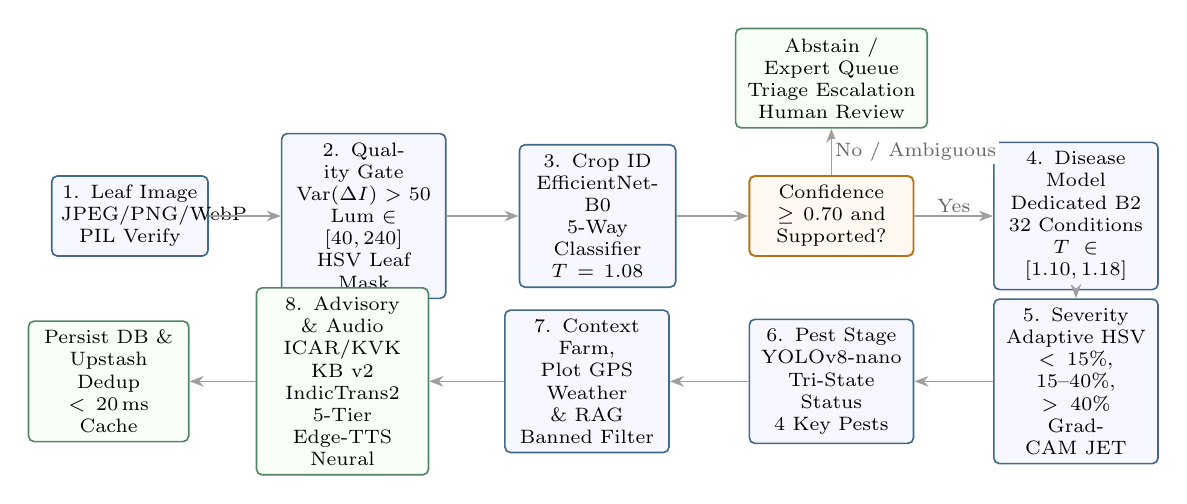
\begin{tikzpicture}[x=1.35cm,y=1cm]
\node[stage,text width=1.75cm] (input) at (0.7,1.4) {1. Leaf Image\\JPEG/PNG/WebP\\PIL Verify};
\node[stage,text width=1.85cm] (quality) at (2.9,1.4) {2. Quality Gate\\$\text{Var}(\Delta I)>50$\\Lum $\in [40,240]$\\HSV Leaf Mask};
\node[stage,text width=1.75cm] (crop) at (5.1,1.4) {3. Crop ID\\EfficientNet-B0\\5-Way Classifier\\$T=1.08$};
\node[decisionbox,text width=1.85cm] (supported) at (7.3,1.4) {Confidence\\$\ge 0.70$ and\\Supported?};
\node[stage,text width=1.85cm] (disease) at (9.6,1.4) {4. Disease Model\\Dedicated B2\\32 Conditions\\$T \in [1.10, 1.18]$};
\node[stage,text width=1.85cm] (severity) at (9.6,-0.7) {5. Severity\\Adaptive HSV\\$<15\%$, $15\text{--}40\%$, $>40\%$\\Grad-CAM JET};
\node[stage,text width=1.85cm] (pest) at (7.3,-0.7) {6. Pest Stage\\YOLOv8-nano\\Tri-State Status\\4 Key Pests};
\node[stage,text width=1.85cm] (context) at (5.0,-0.7) {7. Context\\Farm, Plot GPS\\Weather \& RAG\\Banned Filter};
\node[infra,text width=1.95cm] (advice) at (2.7,-0.7) {8. Advisory \& Audio\\ICAR/KVK KB v2\\IndicTrans2 5-Tier\\Edge-TTS Neural};
\node[infra,text width=1.8cm] (persist) at (0.5,-0.7) {Persist DB \&\\Upstash Dedup\\$<20$\,ms Cache};
\node[infra,text width=2.2cm] (reject) at (7.3,3.15) {Abstain / Expert Queue\\Triage Escalation\\Human Review};
\draw[flowarrow] (input) -- (quality);
\draw[flowarrow] (quality) -- (crop);
\draw[flowarrow] (crop) -- (supported);
\draw[flowarrow] (supported.east) -- node[above,note,fill=white,inner sep=1pt]{Yes} (disease.west);
\draw[flowarrow] (supported.north) -- node[right,note,fill=white,inner sep=1pt]{No / Ambiguous} (reject.south);
\draw[flowarrow] (disease.south) -- (severity.north);
\draw[flowarrow] (severity.west) -- (pest.east);
\draw[flowarrow] (pest.west) -- (context.east);
\draw[flowarrow] (context.west) -- (advice.east);
\draw[flowarrow] (advice.west) -- (persist.east);
\end{tikzpicture}
\caption{The 7-stage AI inference and advisory sequence: incoming leaf imagery passes through OpenCV quality filters, calibrated EfficientNet classifiers, adaptive HSV severity estimation, YOLOv8-nano pest classification, and ICAR/KVK agronomic advisory synthesis with tri-state status handling.}
\label{fig:pipeline}
\end{figure*}

\subsection{Image validation, deduplication, and OpenCV preprocessing}
Client image submissions accept JPEG, PNG, and WebP payloads capped at 10\,MB. Before persistent storage or model computation, two independent layers of binary validation occur:
\begin{enumerate}
  \item \textbf{Magic-Byte and Header Verification:} The payload is verified via PIL's \texttt{Image.verify()} to detect corrupt bitstreams, truncated files, or MIME-spoofing attacks.
  \item \textbf{Cryptographic Deduplication:} A SHA-256 hash of the raw image bytes is calculated. If an identical image has been evaluated within 24 hours for the same user and plot, the backend immediately serves the cached diagnostic result from Upstash Serverless Redis REST (\texttt{sf:dedup:\{hash\}}) in under 20\,ms, avoiding duplicate neural compute.
\end{enumerate}

Images that pass validation are processed through the OpenCV Preprocessing Gate:
\begin{itemize}
  \item \textbf{Laplacian Sharpness Check:} Focus blur is quantified using the variance of the Laplacian operator:
  \begin{equation}
  \sigma^2_{\Delta} = \text{Var}\left( \nabla^2 I \right) = \frac{1}{N}\sum_{x,y} \left( \nabla^2 I(x,y) - \mu_{\Delta} \right)^2
  \end{equation}
  Images exhibiting $\sigma^2_{\Delta} \le 50$ are rejected with code \texttt{failed\_blur}.
  \item \textbf{Luminance Uniformity Check:} Mean pixel luminance in the CIELAB/grayscale domain is required to satisfy $40 \le \mu_L \le 240$; under- or over-exposed images are rejected with \texttt{failed\_lighting}.
  \item \textbf{Foliage ROI Isolation:} Adaptive HSV color segmentation identifies foliage pixel masks ($\text{Hue} \in [25, 85]$). If foliage area occupies less than 5\% of total frame area, the submission is rejected with \texttt{failed\_no\_leaf}.
\end{itemize}

\subsection{Crop identification}
The crop classifier is an EfficientNet-B0 convolutional neural network \cite{ref5} accepting $224 \times 224$ RGB inputs. It outputs a 5-class probability vector spanning Cotton, Groundnut, Pepper Bell, Potato, and Tomato. The model was trained with cosine learning rate scheduling and warmup in PyTorch \cite{ref9}. On the held-out test split of 4,260 images, the model achieves 99.53\% Top-1 accuracy (4,240/4,260 correct), a macro-averaged F1-score of 99.45\%, and a weighted F1-score of 99.50\%. Per-class recall reaches 98.6\% for Cotton, 99.7\% for Groundnut, 99.5\% for Pepper Bell, 100.0\% for Potato, and 99.2\% for Tomato. 

To eliminate overconfidence on field images, post-hoc temperature scaling ($T = 1.08$) is applied to logits:
\begin{equation}
\hat{p}_i = \frac{\exp(z_i / T)}{\sum_j \exp(z_j / T)}
\end{equation}
Calibration reduces the Expected Calibration Error (ECE) from 0.0210 to 0.0072 with a final Brier score of 0.0076 \cite{ref12}. Controlled-environment accuracy is 99.65\% (2,855/2,865), while in-situ field imagery achieves 99.35\% (1,385/1,395).

\subsection{Decision routing and confidence gating}
The Decision Engine enforces an empirical confidence gating threshold ($\tau_{\text{crop}} = 0.70$, dynamically configurable via \texttt{sf:config:thresholds}). If the top predicted crop confidence falls below $\tau_{\text{crop}}$ or the predicted label does not match the 5 supported agricultural species, the engine safely bypasses disease classification, marks the disease finding as \texttt{unsupported\_crop}, and automatically triggers an agronomist triage review (\texttt{ensure\_expert\_review()}). When confidence meets or exceeds $\tau_{\text{crop}}$, the engine routes the normalized leaf tensor to the designated crop-specific disease model.

\subsection{Crop-specific disease classifiers}
Rather than employing a single diluted multi-crop classifier, the platform uses 5 dedicated EfficientNet-B2 neural networks, one for each supported crop. This modular architecture allows independent model retraining and evaluation across 32 total phytopathological conditions:
\begin{itemize}
  \item \textbf{Cotton (4 conditions)}: Bacterial Blight, Curl Virus, Fusarium Wilt, Healthy.
  \item \textbf{Groundnut (4 conditions)}: Early Leaf Spot (Tikka), Late Leaf Spot, Rust, Healthy.
  \item \textbf{Pepper Bell (3 conditions)}: Bacterial Spot, Cercospora Leaf Spot, Healthy.
  \item \textbf{Potato (4 conditions)}: Early Blight, Late Blight, Black Scurf, Healthy.
  \item \textbf{Tomato (10 conditions)}: Bacterial Spot, Early Blight, Late Blight, Leaf Mold, Septoria Leaf Spot, Spider Mites (Two-spotted spider mite damage), Target Spot, Yellow Leaf Curl Virus, Mosaic Virus, Healthy.
  \item \textbf{Cross-crop controls (7 classes)}: Background, abiotic leaf scorch, and nutrient deficiencies.
\end{itemize}
Each disease classifier utilizes tailored post-hoc logit scaling ($T \in [1.10, 1.18]$) in \texttt{config.yaml}. Predictions falling below $\tau_{\text{disease}} = 0.70$ automatically trigger expert escalation.

\subsection{Severity estimation and visual saliency}
Infection severity is estimated using an adaptive HSV color segmentation heuristic that quantifies the visible necrotic and chlorotic lesion area as a percentage of total segmented leaf area:
\begin{equation}
\text{Severity}_{\text{pct}} = \frac{\text{Area}(\text{Lesion Mask})}{\text{Area}(\text{Foliage Mask})} \times 100
\end{equation}
The percentage is mapped into standardized agronomic tiers: \textit{Healthy} (0\%), \textit{Low} ($<15\%$), \textit{Medium} ($15\%$--$40\%$), and \textit{High} ($>40\%$). 

To eliminate false-positive lesion artifacts on healthy crops, a classification-guided suppression rule checks the disease classifier output: if the healthy class confidence exceeds 0.85, lesion contours are suppressed, forcing severity to 0\% and bucket to \textit{Healthy}. Saliency visualization is generated via Grad-CAM at the final convolutional layer of the EfficientNet-B2 backbone, rendered as a JET colormap overlay to highlight diagnostic lesion margins (see Fig.~\ref{fig:saliency-and-vernacular}(a)).

\subsection{Pest classification with tri-state status}
Agricultural insect damage is classified using an Ultralytics YOLOv8-nano classification network \cite{ref7} trained on four major crop pests: Aphid (\textit{Aphis gossypii}), Armyworm (\textit{Spodoptera frugiperda}), Leaf Miner (\textit{Liriomyza}), and Spider Mite (\textit{Tetranychus urticae}). 

The pipeline strictly enforces a tri-state status contract to avoid false assumptions:
\begin{itemize}
  \item \texttt{pest\_detected}: One or more pest categories detected above 0.50 confidence, returning ranked labels and probabilities.
  \item \texttt{no\_pests\_detected}: Model successfully executed with foliage verified free of target pest visual markers.
  \item \texttt{unavailable}: Model weights unconfigured or execution bypassed; client interfaces gracefully render an informative fallback pill without degrading primary disease results.
\end{itemize}

\subsection{Agronomic advisory, RAG guardrails, and vernacular synthesis}
Advisory generation prioritizes safety, determinism, and regional compliance:
\begin{enumerate}
  \item \textbf{ICAR/KVK Grounded Knowledge Base:} The primary advisory engine is grounded in a deterministic, peer-reviewed agronomic database (\texttt{advisory\_kb.json} v2) encompassing 56 condition profiles and 155 disease aliases formulated according to Indian Council of Agricultural Research (ICAR) and Krishi Vigyan Kendra (KVK) guidelines. It executes with sub-millisecond CPU latency and zero API cost.
  \item \textbf{RAG Safety Guardrails:} When cloud acceleration is active (Groq Llama-3.3-70B or local Qwen2.5-1.5B), a TF-IDF cosine-similarity retriever injects approved chemical dosages and cultural practices into the system prompt while strictly censoring prohibited substances (Endosulfan, Monocrotophos, Methyl Parathion, Phorate, Carbaryl) and enforcing pre-harvest intervals (PHI). Structured outputs are validated against a Pydantic schema (\texttt{immediate\_action}, \texttt{treatment}, \texttt{prevention}, \texttt{monitoring}) and unconditionally appended with an agronomic safety disclaimer.
  \item \textbf{Multi-Tier Zero-Hang Translation:} The advisory is translated into Hindi and Gujarati across a 5-tier fallback cascade: (Tier~1) 400+ domain term cache; (Tier~2) sentence splitting; (Tier~3) Groq Llama translation; (Tier~4) Google Translate with 3.5\,s timeout; (Tier~5) local IndicTrans2-dist-200M Seq2Seq decoding. Pre-translations are dispatched via \texttt{FastAPI.BackgroundTasks} and cached in PostgreSQL \texttt{entity\_translations}.
  \item \textbf{Neural Speech Narration:} Synchronized spoken audio is generated via Microsoft Edge-TTS neural models (\texttt{hi-IN-SwaraNeural}, \texttt{gu-IN-DhwaniNeural}, \texttt{en-IN-NeerjaNeural}), serialized as MP3, and cached under \texttt{data/audio} or Supabase Object Storage for instant playback.
\end{enumerate}

% ---------------- Section ----------------
\section{Backend API and Application Workflows}
\subsection{API conventions and gateway architecture}
The API gateway is implemented using FastAPI \cite{ref8} and deployed on Render as an asynchronous web service managed by Gunicorn and Uvicorn workers. All endpoints adhere to REST principles and the platform API specification \cite{ref1}: structured JSON bodies (\texttt{application/json}), multipart image uploads (\texttt{multipart/form-data}), and standard HTTP status codes. All production routes are mounted under the canonical \texttt{/api/v1} prefix, with legacy unversioned paths retained as compatibility aliases. 

To eliminate cold-start timeouts on low-cost hosting, the backend features an asynchronous non-blocking lifespan: database connectivity verification is pushed to background tasks to achieve instantaneous port binding ($<1$\,s). Rate limiting is enforced per remote client IP via \texttt{slowapi} token buckets (e.g., 5 requests/min for login, 20 requests/min for inference).

\subsection{Core endpoint groups}
\begin{table*}[!t]
\centering
\footnotesize
\caption{Production REST API Endpoints and Service Responsibilities}
\label{tab:endpoints}
\begin{tabularx}{\textwidth}{l >{\raggedright\arraybackslash\ttfamily}p{6.6cm} X}
\toprule
\textbf{Method} & \textbf{Endpoint / Path} & \textbf{Implementation Details and Operational Purpose}\\
\midrule
POST & /api/v1/auth/register & Registers farmer/expert account with Argon2id password hashing and farm profile metadata.\\
POST & /api/v1/auth/login & Authenticates via email/phone; issues 30-min JWT access token and 30-day HttpOnly refresh cookie.\\
POST & /api/v1/auth/guest & 1-tap onboarding issuing ephemeral session (\texttt{role: farmer}) for friction-free diagnostic access.\\
POST & /api/v1/auth/refresh & Database-backed token rotation in PostgreSQL \texttt{refresh\_tokens} table with Token Family Reuse Detection.\\
POST & /api/v1/auth/logout & Revokes active refresh token and clears HttpOnly cookie.\\
POST & /api/v1/predict & Validates PIL magic-bytes, checks Upstash dedup cache ($<$20\,ms), and runs 7-stage vision pipeline.\\
GET & /api/v1/predictions/\{id\} & Retrieves completed diagnostic result with crop, disease, severity, pests, advisory, and provenance.\\
POST & /api/v1/predictions/\{id\}/rescan & Links a newly captured specimen scan to an existing prediction history chain.\\
POST & /api/v1/predictions/\{id\}/request-expert & Escalates diagnostic result to agronomist review triage queue.\\
POST & /api/v1/predictions/\{id\}/translate & Triggers on-demand translation of advisory recommendation into target language.\\
GET / POST & /api/v1/farm \textnormal{and} /farm/plots & Manages farm boundaries, plots, and GeoJSON polygons with geodesic acreage and Shapely validation.\\
GET & /api/v1/weather & Returns live OpenWeatherMap observation (30-min Upstash grid cache) with localized advisory.\\
GET & /api/v1/alerts & Fetches user alert notifications (weather microclimate alerts, agronomist verification updates).\\
GET & /api/v1/expert/queue & Retrieves unverified cases awaiting agronomist review with signed image URLs.\\
POST & /api/v1/expert/reviews/\{id\} & Submits triage review (approve, override label/severity, or request rescan); creates \texttt{DatasetCandidate}.\\
POST & /api/v1/internal/cron/* & Multi-region QStash webhook receiver (\texttt{Upstash-Signature} validated) for weather risks and blob purge.\\
POST & /api/v1/tts/synthesize & Synthesizes vernacular speech narration using Microsoft Edge-TTS neural models.\\
GET & /api/v1/admin/metrics & Exposes P95 processing duration, feedback vs.\ expert accuracy, confidence histograms, and drift telemetry.\\
POST & /api/v1/admin/mlops/export & Builds zero-leakage dataset export using SHA-256 spatial plot hashing and 70/30 replay buffer mixing.\\
GET / POST & /api/v1/admin/models/* & Inspects model health on disk, enforces minimum test-accuracy promotion gates, and executes rollback.\\
\bottomrule
\end{tabularx}
\end{table*}

\begin{figure}[!t]
\centering
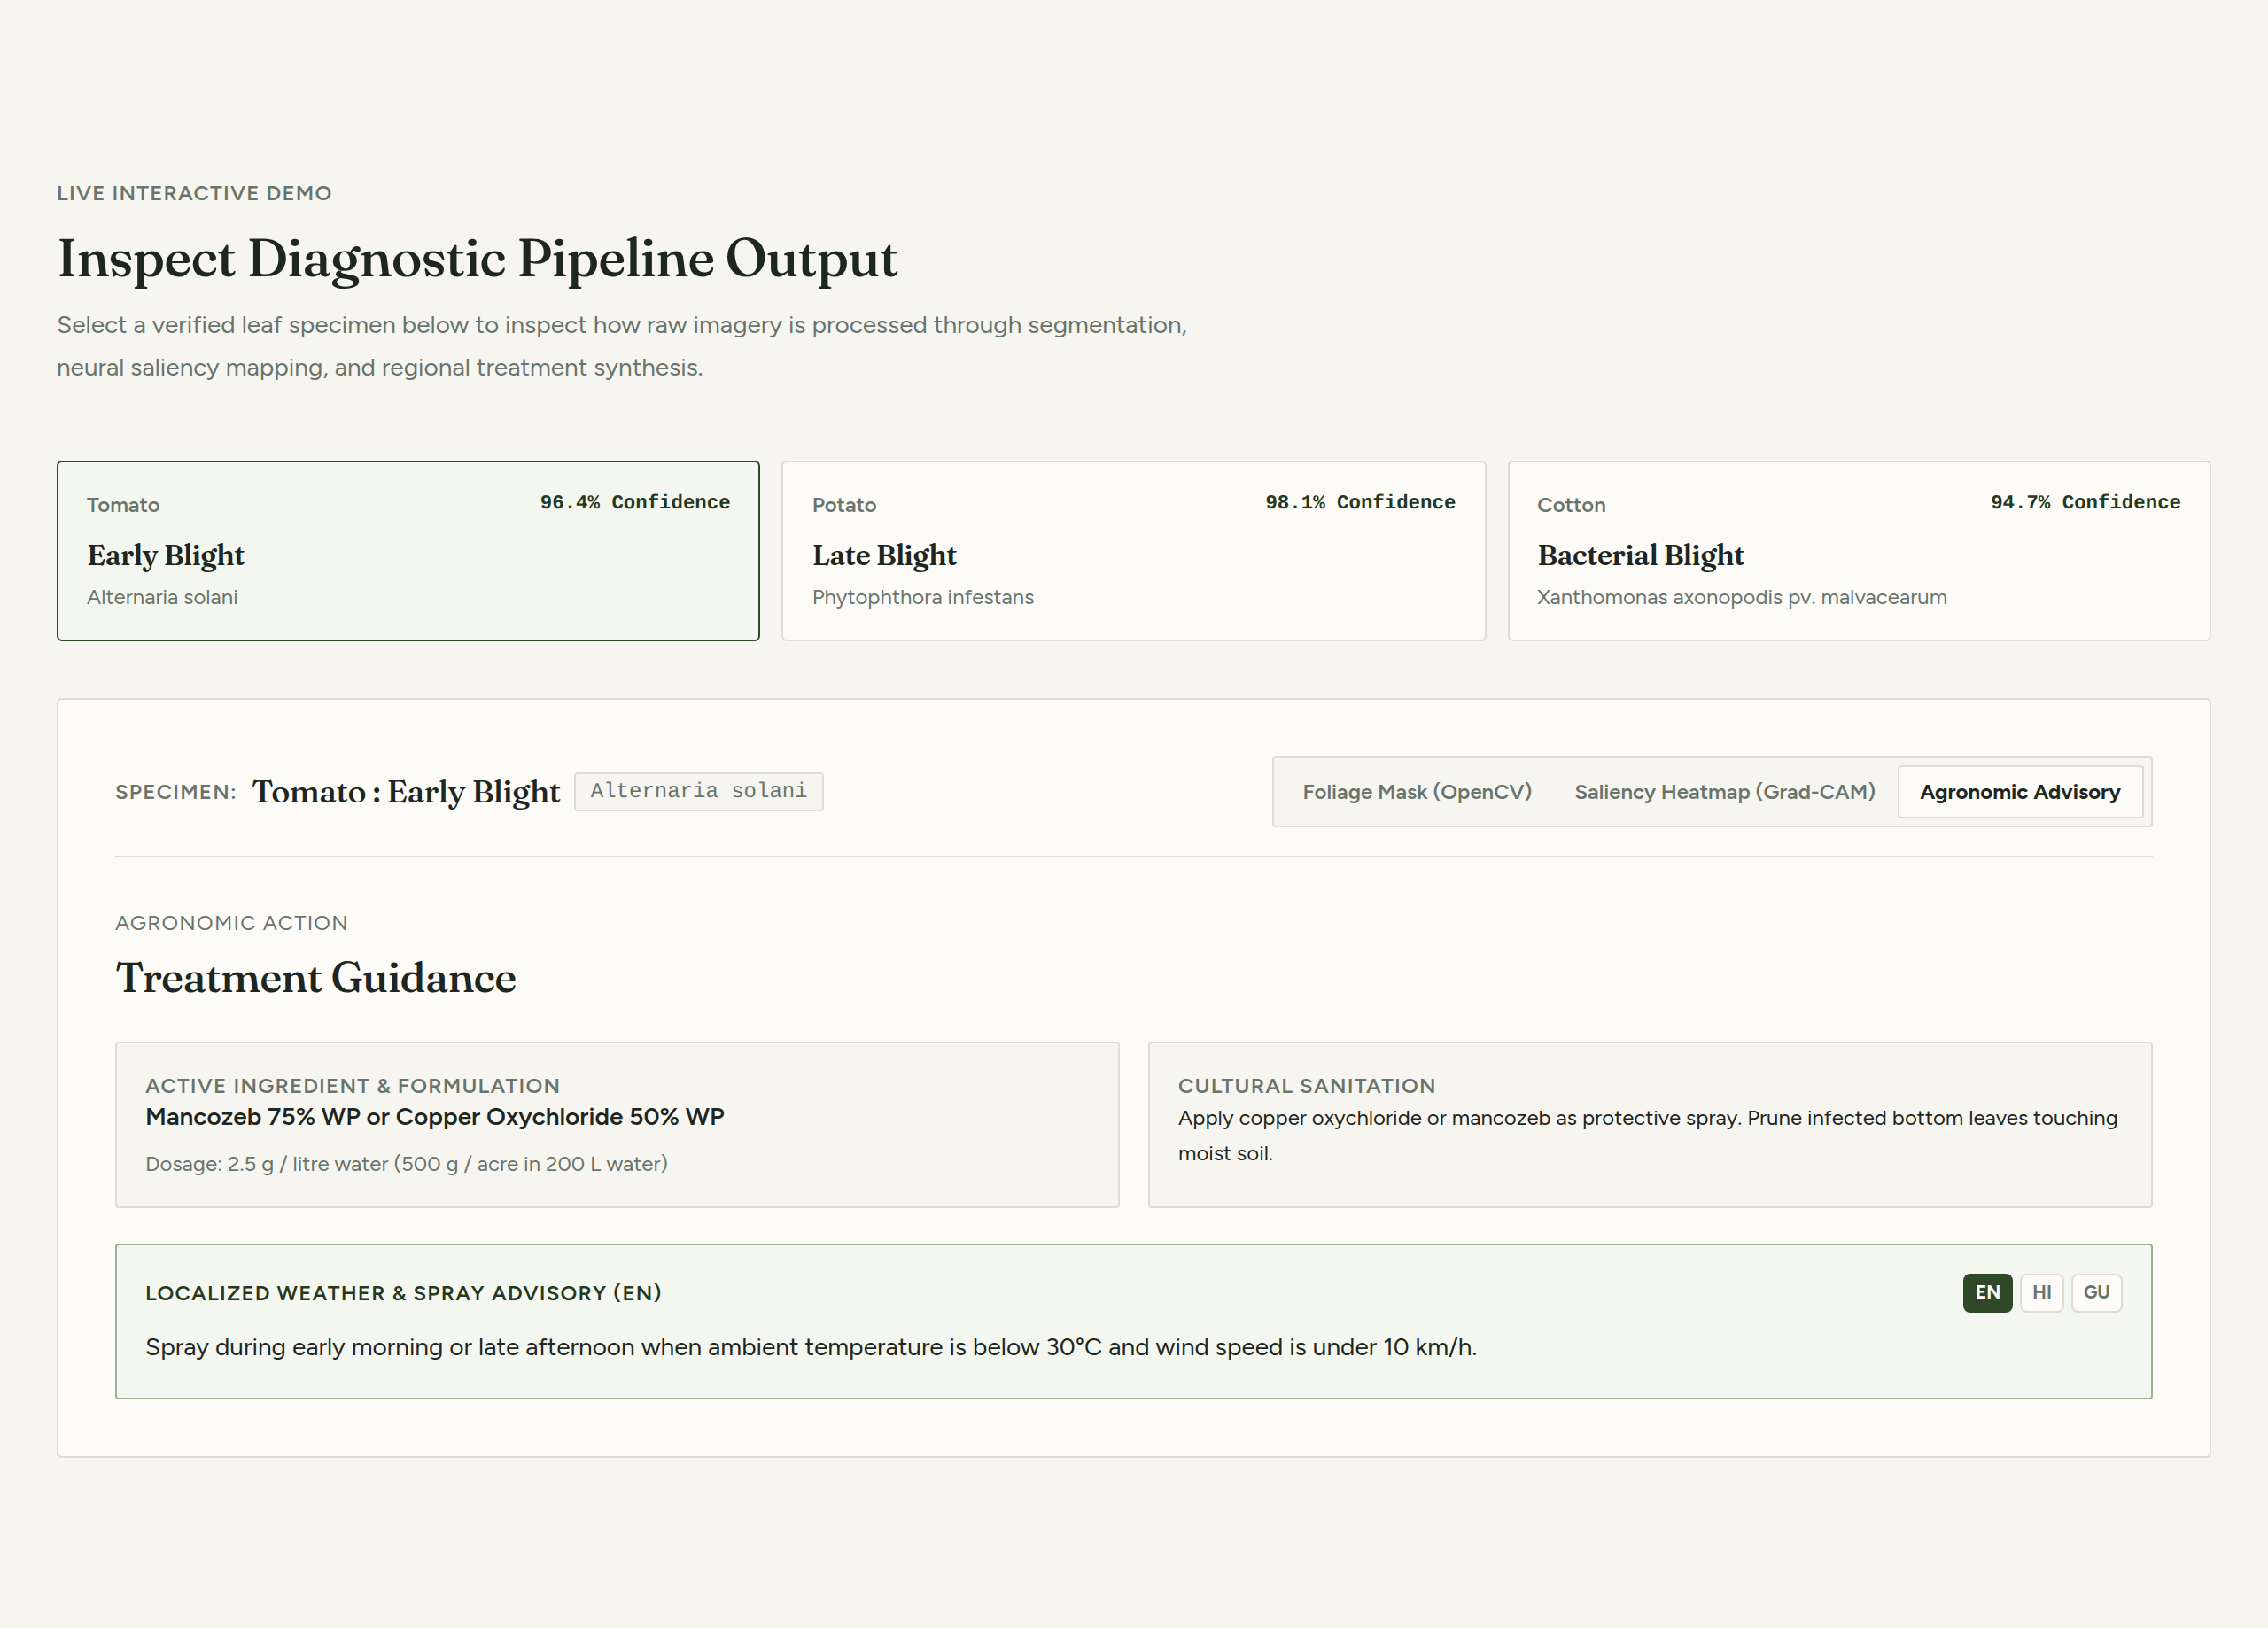
\includegraphics[width=\columnwidth]{screenshots/10_demo_workbench_advisory_en.png}
\caption{Web client diagnostic output displaying specimen condition (Tomato Early Blight, 96.4\% confidence), active chemical formulation dosage, cultural sanitation guidance, and localized weather spray advisory.}
\label{fig:prediction-advisory}
\end{figure}

\subsection{Keyless GIS farm and plot boundary mapping}
Agricultural parcel mapping in the web client (\texttt{FarmSettingsPage.tsx}) is implemented using open-source \textbf{Leaflet} (\texttt{react-leaflet}) rather than proprietary map providers. This architecture guarantees keyless deployment with zero external API quotas or billing:
\begin{itemize}
  \item \textbf{Dual Base-Map Switching:} Farmers toggle seamlessly between OpenStreetMap (standard street map) and Esri World Imagery (high-resolution satellite view) to distinguish field vegetation and furrows.
  \item \textbf{Interactive Polygon Editing:} Farmers plot polygon boundaries by clicking vertices. The canvas dynamically displays draggable circular vertex markers, allows intermediate vertex insertion along perimeters, and supports double-click vertex removal.
  \item \textbf{Geodesic Acreage Telemetry:} Boundary geometry is projected onto geodesic coordinates in real time, calculating field surface area in acres and hectares.
  \item \textbf{Geometric Integrity Gate:} The backend validates submitted GeoJSON polygons via Shapely (\texttt{\_validate\_geojson\_polygon}), verifying closed linear rings ($\text{ring}[0] = \text{ring}[-1]$), coordinate boundary limits ($-180 \le \lambda \le 180, -90 \le \phi \le 90$), and absence of self-intersections. In-process ray casting (\texttt{\_plot\_inside\_farm}) enforces that plots remain strictly bounded within parent farm boundaries.
  \item \textbf{Mobile Field Boundary Snapping:} The Flutter mobile client provides a center-crosshair boundary drawing interface with magnetic edge snapping, auto-projecting vertices placed outside the farm boundary to the nearest edge coordinate.
\end{itemize}

\subsection{Prediction lifecycle and agronomist triage workflow}
\begin{figure*}[!t]
\centering
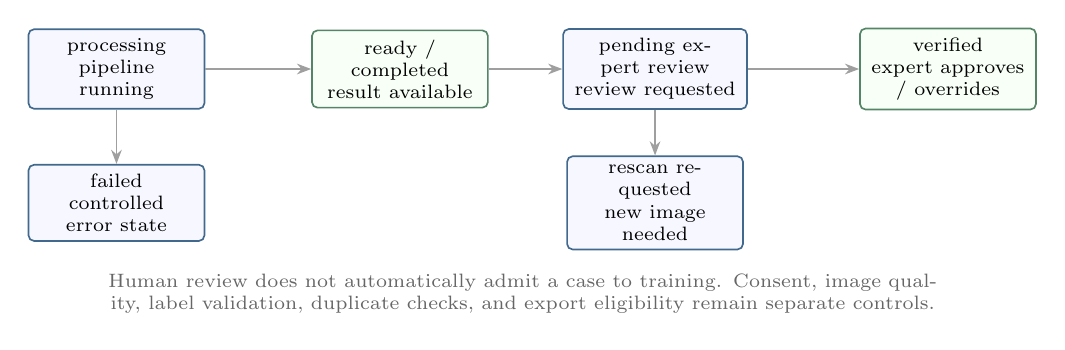
\begin{tikzpicture}[x=1.2cm,y=1cm]
\node[stage,text width=2.0cm] (processing) at (1.0,1.2) {processing\\pipeline running};
\node[infra,text width=2.0cm] (ready) at (4.0,1.2) {ready / completed\\result available};
\node[stage,text width=2.0cm] (failed) at (1.0,-0.5) {failed\\controlled error state};
\node[stage,text width=2.1cm] (review) at (6.7,1.2) {pending expert review\\review requested};
\node[infra,text width=2.0cm] (verified) at (9.8,1.2) {verified\\expert approves / overrides};
\node[stage,text width=2.0cm] (rescan) at (6.7,-0.5) {rescan requested\\new image needed};
\draw[flowarrow] (processing) -- (ready);
\draw[flowarrow] (processing.south) -- (failed.north);
\draw[flowarrow] (ready) -- (review);
\draw[flowarrow] (review) -- (verified);
\draw[flowarrow] (review.south) -- (rescan.north);
\node[note,text width=12cm] at (5.3,-1.65) {Human review does not automatically admit a case to training. Consent, image quality, label validation, duplicate checks, and export eligibility remain separate controls.};
\end{tikzpicture}
\caption{Prediction and expert-review states documented in the API reference. Transitions are illustrative; verify exact state enums against the deployed API schema.}
\label{fig:lifecycle}
\end{figure*}

Fig.~\ref{fig:lifecycle} depicts the operational state machine governing scan progression. Every submitted specimen begins in state \texttt{processing}. Upon successful pipeline completion, the record transitions to \texttt{ready}. If any model stage fails or quality checks reject the image, a controlled transition to \texttt{failed} occurs with diagnostic failure details.

When an automated diagnosis exhibits low confidence ($\tau < 0.70$), indicates an unsupported crop, or when a farmer explicitly requests verification, \texttt{ensure\_expert\_review()} transactionally creates an \texttt{ExpertReview} record and updates the prediction state to \texttt{pending\_expert\_review}. 

The Agronomist Review Console provides a dedicated triage environment:
\begin{enumerate}
  \item \textbf{Atomic Lease Locking:} To prevent collision when multiple agronomists review cases simultaneously, claiming a case sets an atomic 15-minute lease lock.
  \item \textbf{Side-by-Side Saliency Verification:} Agronomists inspect raw leaf images alongside Grad-CAM attention heatmaps and OpenCV foliage masks (see Fig.~\ref{fig:saliency-and-vernacular}(a)).
  \item \textbf{Triage Actions:} The expert can select one of three actions:
  \begin{itemize}
    \item \textit{Approve Finding}: Confirms the automated diagnosis; updates status to \texttt{verified}.
    \item \textit{Override / Correct Findings}: Overrides the disease label or severity percentage; the database atomically updates \texttt{prediction.disease} and flags the SQLAlchemy JSON column as modified.
    \item \textit{Request Rescan}: Flags poor lighting or leaf occlusion, moving prediction status to \texttt{rescan\_requested} and dispatching an in-app alert to the farmer.
  \end{itemize}
  \item \textbf{Continuous Retraining Loop:} Flagging a case with \texttt{add\_to\_retraining=true} persists an entry into the \texttt{DatasetCandidate} table, capturing the verified label and image provenance for scheduled MLOps export.
\end{enumerate}

\subsection{Mobile offline scouting and vernacular TTS}
The Flutter mobile application (\texttt{FarmerShell}) is tailored specifically for rural field operations:
\begin{itemize}
  \item \textbf{Offline-First SQLite Queue:} In remote regions with intermittent or absent cellular connectivity, captured specimen scans and plot associations are stored in an offline SQLite database (\texttt{OfflineQueueDb}). A background synchronization service (\texttt{SyncService}) drains queued jobs with exponential backoff once network connectivity is restored.
  \item \textbf{Dual TTS Narration:} Spoken audio guidance is synthesized via the cloud Microsoft Edge-TTS service, with graceful fallback to on-device text-to-speech engine (\texttt{flutter\_tts}) when offline.
\end{itemize}

\begin{figure*}[!t]
\centering
\begin{minipage}{0.49\textwidth}
  \centering
  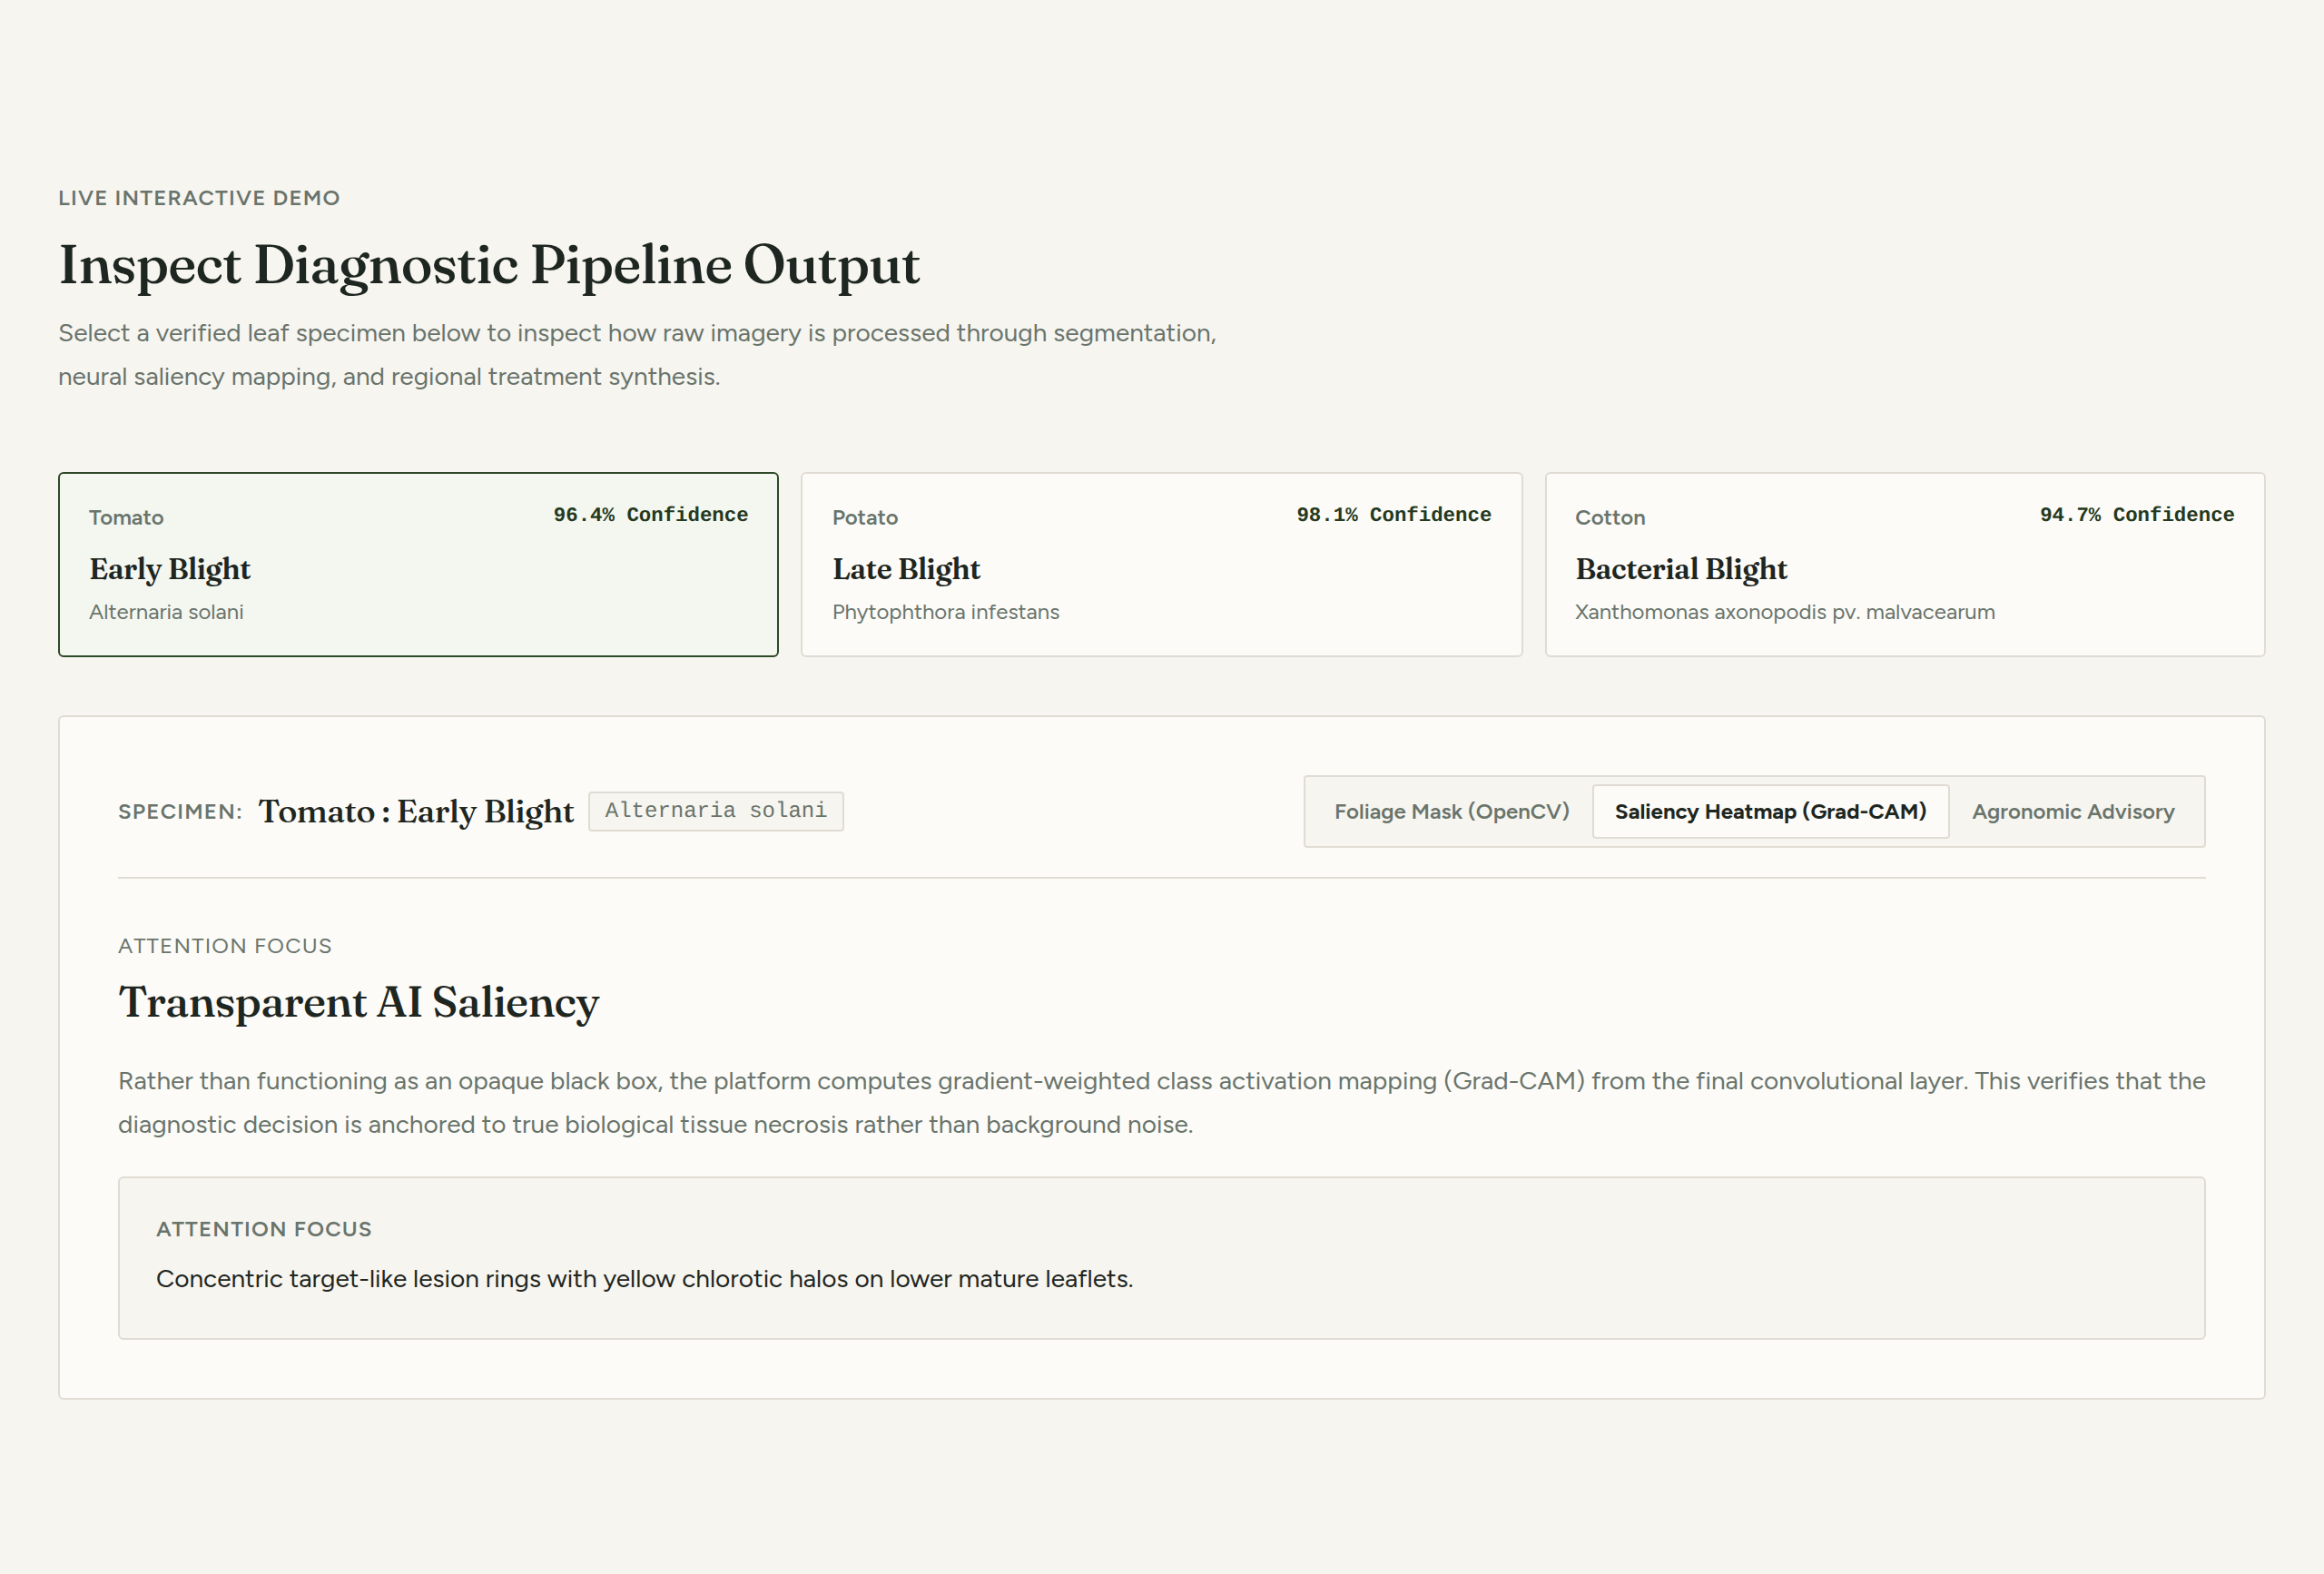
\includegraphics[width=\linewidth]{screenshots/09_demo_workbench_saliency.png}
  \caption*{(a) Grad-CAM visual attention verification targeting lesion halos.}
\end{minipage}\hfill
\begin{minipage}{0.49\textwidth}
  \centering
  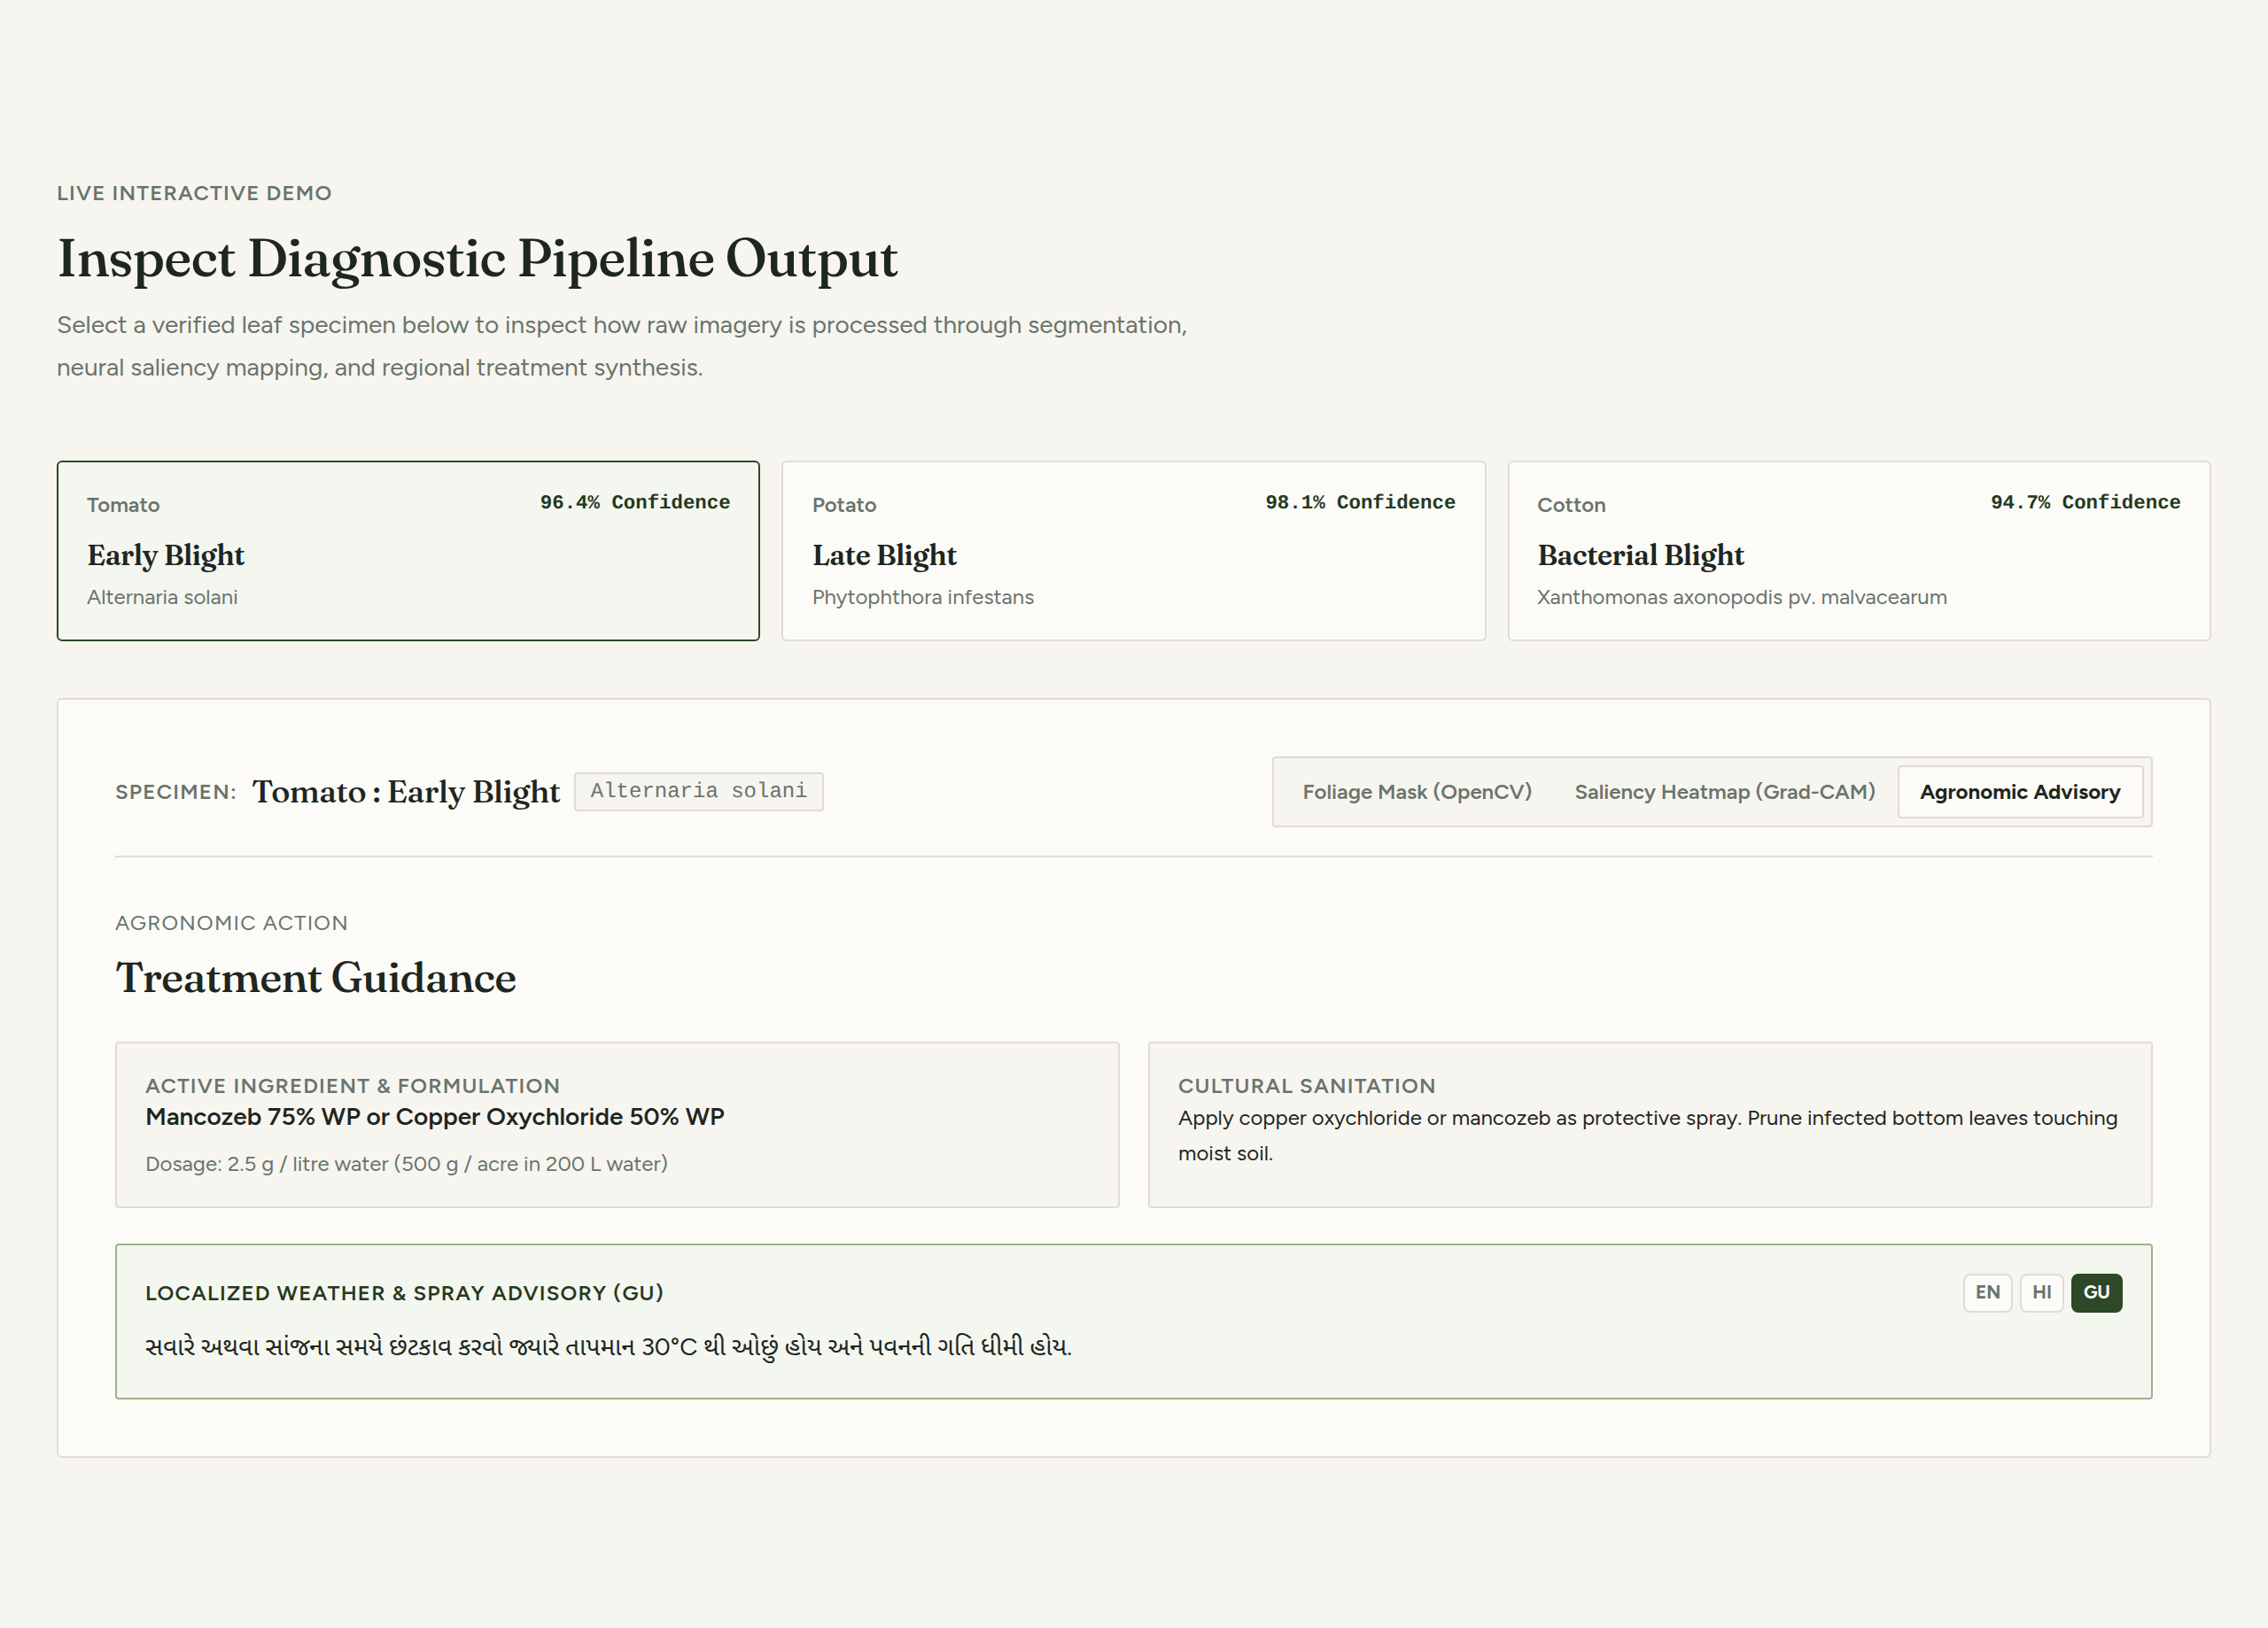
\includegraphics[width=\linewidth]{screenshots/11_demo_workbench_advisory_gujarati.png}
  \caption*{(b) Vernacular regional advisory dynamically translated into Gujarati.}
\end{minipage}
\caption{Explainability and regional accessibility: (a) Grad-CAM attention focuses on concentric necrotic halos rather than leaf boundaries; (b) Trilingual localization allows regional farmers to receive actionable advice in Gujarati.}
\label{fig:saliency-and-vernacular}
\end{figure*}

% ---------------- Section ----------------
\section{Security, Privacy and Access Control}
\subsection{Authentication and token rotation}
User authentication implements dual-token bearer architecture combined with database-backed token lifecycle management as specified in the authentication reference \cite{ref2}:
\begin{enumerate}
  \item \textbf{Token Lifecycle:} Short-lived HS256 JWT access tokens (30-minute validity) are transmitted via the \texttt{Authorization: Bearer} header. Long-lived refresh tokens (30-day validity) are stored inside an \texttt{HttpOnly}, \texttt{SameSite=Strict} cookie. In production, the \texttt{Secure} flag is strictly enforced.
  \item \textbf{Password Hashing:} Credentials are protected using the memory-hard Argon2id algorithm via \texttt{pwdlib[argon2]}, providing robust resistance against GPU/ASIC rainbow-table attacks.
  \item \textbf{Production Secret Verification:} In \texttt{backend/src/app/core/config.py}, the server executes an unconditional startup validation guard that halts execution if \texttt{JWT\_SECRET\_KEY} matches the default development string. The development-convenience header bypass (\texttt{X-User-ID}) is strictly restricted to \texttt{DEBUG=True} or \texttt{ENVIRONMENT="test"}.
  \item \textbf{Database-Backed Token Family Reuse Detection:} Refresh tokens are tracked in the PostgreSQL \texttt{refresh\_tokens} table. Every call to \texttt{POST /api/v1/auth/refresh} revokes the presented refresh token and issues a new token pair. If an already-revoked refresh token is re-submitted (indicating token theft or replay), the system triggers Token Family Reuse Detection, revoking all active sessions belonging to that token family immediately with HTTP 401.
  \item \textbf{Friction-Free Guest Mode:} To lower adoption barriers for first-time farmers in the field, \texttt{POST /api/v1/auth/guest} provisions an ephemeral session (\texttt{role: farmer}, prefixed with \texttt{guest\_}), enabling instant leaf diagnosis without mandatory registration.
\end{enumerate}

\subsection{Database triggers and dynamic remote config security}
Cross-service synchronization between external identity providers and internal PostgreSQL models is safeguarded through database-level isolation:
\begin{itemize}
  \item \textbf{Hardened Supabase Auth Trigger:} Alembic migration \texttt{0003\_supabase\_auth\_sync.py} establishes a synchronized trigger function (\texttt{handle\_new\_user()}) on \texttt{auth.users}. The trigger is secured with \texttt{SECURITY DEFINER SET search\_path = ''} to prevent search-path hijacking. It forces newly created user roles strictly to \texttt{farmer}, explicitly ignoring any client-supplied role parameters in \texttt{raw\_user\_meta\_data}. Conflict handling on duplicate insertion strictly omits role modification to prevent privilege escalation.
  \item \textbf{Remote Config Backend URL Locking:} The Flutter mobile client resolves its API endpoint dynamically via \texttt{RemoteConfigService}, fetching the active base URL from the Supabase \texttt{public.app\_config} table via PostgREST. The table is protected by PostgreSQL Row-Level Security (RLS) with public read-only access for anonymous and authenticated users; write access is restricted to database administrators. All client-side server configuration dialogs and developer URL overrides have been eliminated from production builds, preventing MITM server redirection.
\end{itemize}

\subsection{Role-based access control}
The platform enforces a strict hierarchical role structure:
\begin{equation}
\text{Admin} \supset \text{Expert} \supset \text{Farmer}
\end{equation}
Table~\ref{tab:rbac} details the authorization matrix enforced through FastAPI dependency injections (\texttt{require\_expert\_role}, \texttt{require\_admin\_role}).

\begin{table}[!t]
\centering
\caption{Role-based capability and access control matrix}
\label{tab:rbac}
\begin{tabularx}{\columnwidth}{p{2.6cm}XXX}
\toprule
\textbf{Capability} & \textbf{Farmer} & \textbf{Expert} & \textbf{Admin}\\
\midrule
Personal scan and history & Yes & Yes & Yes\\
Personal farm/plot boundaries & Yes & Yes & Yes\\
Weather and microclimate alerts & Yes & Yes & Yes\\
Triage review queue and actions & No & Yes & Yes\\
Farmer feedback audit & No & Yes & Yes\\
User and role management & No & No & Yes\\
Dynamic threshold configuration & No & No & Yes\\
MLOps dataset candidate export & No & No & Yes\\
Model registry and promotion & No & No & Yes\\
Platform-wide media access & No & No & Yes\\
\bottomrule
\end{tabularx}
\end{table}

\subsection{Media access control and short-lived signed URLs}
Raw leaf photos, Grad-CAM attention heatmaps, and audio narrations represent sensitive agricultural assets. Public bucket access is disabled. All media access is brokered through time-bounded signed URLs (default 900\,s / 15\,min) generated by \texttt{SupabaseStorageBackend}:
\begin{itemize}
  \item A farmer can only request signed media URLs for their own scans (\texttt{user\_id == current\_user.id}).
  \item An agronomist can only access media for cases currently pending in the triage queue (\texttt{pending\_expert\_review}) or assigned to their account.
  \item Administrators hold platform-wide signed URL creation privileges. Cross-user media access attempts are rejected with HTTP 403 Forbidden.
\end{itemize}

\subsection{Administrative anti-lockout safeguards}
Two deterministic database-level invariants protect platform administrative access during role modifications via \texttt{PATCH /api/v1/admin/users/\{id\}/role}:
\begin{enumerate}
  \item \textbf{Self-Demotion Prevention:} An administrator is prohibited from demoting their own account to expert or farmer, preventing accidental administrative loss.
  \item \textbf{Last-Administrator Guard:} The endpoint verifies the active count of administrators; if an update would reduce the administrator count to zero, the request is rejected with HTTP 400.
\end{enumerate}

% ---------------- Section ----------------
\section{Model Training, MLOps, and Retraining Lifecycle}
\subsection{Training environment and transfer learning recipe}
The model training pipeline is implemented in Python 3.12 using PyTorch \cite{ref9}, torchvision, and scikit-learn, with GPU acceleration on NVIDIA CUDA hardware as documented in the MLOps training guide \cite{ref3}. Training uses a two-phase transfer learning schedule:
\begin{enumerate}
  \item \textbf{Warmup Phase:} The convolutional feature extractor backbone is frozen. Only the newly attached classification head is trained for 2--3 epochs at a learning rate of $2 \times 10^{-4}$ (AdamW optimizer) to stabilize gradient magnitudes.
  \item \textbf{Fine-Tuning Phase:} The entire backbone is unfrozen and trained with a cosine annealing learning rate schedule down to $1 \times 10^{-6}$, applying class-balanced cross-entropy loss with label smoothing ($\epsilon = 0.1$) to prevent over-fitting on rare disease classes.
\end{enumerate}

\subsection{Spatial plot-hashed dataset export and zero data leakage}
In agricultural vision systems, repeated photo capture of the same plant or plot across consecutive days poses a severe risk of data leakage if images are partitioned randomly. The platform's MLOps export engine (\texttt{POST /api/v1/admin/mlops/export}) resolves this through three architectural controls:
\begin{enumerate}
  \item \textbf{Deterministic Spatial Plot Hashing:} Dataset candidates are partitioned across train (70\%), validation (15\%), and test (15\%) sets using SHA-256 partition hashing strictly keyed on \texttt{plot\_id}:
  \begin{equation}
  h = \text{SHA256}(\text{plot\_id}) \pmod{100}
  \end{equation}
  Splits are assigned by threshold: $h < 70 \implies \text{train}$, $70 \le h < 85 \implies \text{val}$, and $h \ge 85 \implies \text{test}$. This guarantees zero spatial leakage: all scans of a specific field remain quarantined to a single split.
  \item \textbf{Replay Buffer Mixing:} To prevent catastrophic forgetting when retraining on newly verified field corrections, the export engine enforces a configurable replay buffer ratio (default 30\%, range 0.0 to 0.95), automatically blending curated baseline benchmark samples with newly verified candidates.
  \item \textbf{EXIF Scrubbing and Multi-Format Archiving:} Image metadata (GPS coordinates, device IDs) is scrubbed to preserve farmer privacy. The engine supports five archive formats: PyTorch Folder hierarchy (\texttt{images/<split>/<class\_label>/}), JSON Manifest, YOLO format, CSV tabular index, and TFRecord, supporting both raw and preprocessed (224 $\times$ 224 normalized OpenCV) targets.
\end{enumerate}

\begin{figure*}[!t]
\centering
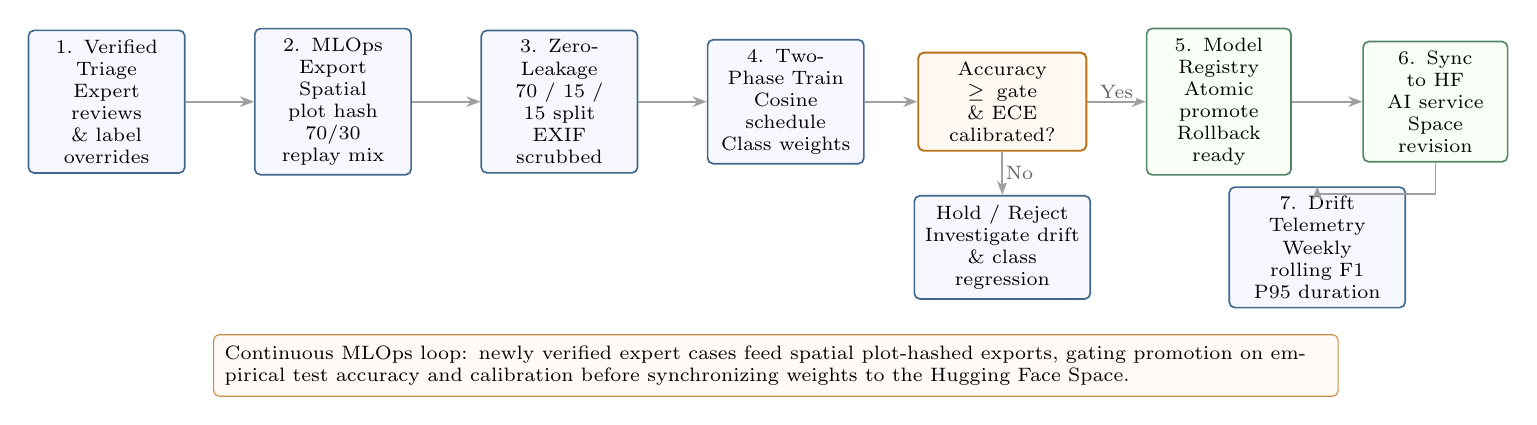
\begin{tikzpicture}[x=1.25cm,y=1cm]
\node[stage,text width=1.75cm] (feedback) at (0.7,1.2) {1. Verified Triage\\Expert reviews\\\& label overrides};
\node[stage,text width=1.75cm] (export) at (3.0,1.2) {2. MLOps Export\\Spatial plot hash\\70/30 replay mix};
\node[stage,text width=1.75cm] (split) at (5.3,1.2) {3. Zero-Leakage\\70 / 15 / 15 split\\EXIF scrubbed};
\node[stage,text width=1.75cm] (train) at (7.6,1.2) {4. Two-Phase Train\\Cosine schedule\\Class weights};
\node[decisionbox,text width=1.9cm] (gate) at (9.8,1.2) {Accuracy $\ge \text{gate}$\\\& ECE calibrated?};
\node[infra,text width=1.6cm] (registry) at (12.0,1.2) {5. Model Registry\\Atomic promote\\Rollback ready};
\node[infra,text width=1.6cm] (deploy) at (14.2,1.2) {6. Sync to HF\\AI service\\Space revision};
\node[stage,text width=2.0cm] (hold) at (9.8,-0.65) {Hold / Reject\\Investigate drift\\\& class regression};
\node[stage,text width=2.0cm] (monitor) at (13.0,-0.65) {7. Drift Telemetry\\Weekly rolling F1\\P95 duration};
\draw[flowarrow] (feedback) -- (export);
\draw[flowarrow] (export) -- (split);
\draw[flowarrow] (split) -- (train);
\draw[flowarrow] (train) -- (gate);
\draw[flowarrow] (gate.east) -- node[above,note,fill=white,inner sep=1pt]{Yes} (registry.west);
\draw[flowarrow] (gate.south) -- node[right,note,fill=white,inner sep=1pt]{No} (hold.north);
\draw[flowarrow] (registry) -- (deploy);
\draw[flowarrow] (deploy.south) -- ++(0,-0.4) -| (monitor.north);
\node[draw=sfamber!80,fill=orange!4,rounded corners=2pt,text width=14.0cm,align=left,inner sep=4pt,font=\scriptsize] at (7.5,-2.15) {Continuous MLOps loop: newly verified expert cases feed spatial plot-hashed exports, gating promotion on empirical test accuracy and calibration before synchronizing weights to the Hugging Face Space.};
\end{tikzpicture}
\caption{End-to-end MLOps retraining and promotion lifecycle: verified agronomist corrections are exported with zero spatial leakage, evaluated against quantitative gates, registered, and promoted atomically.}
\label{fig:mlops}
\end{figure*}

\subsection{Model registry and atomic promotion gates}
The Model Registry (\texttt{model\_registry.json}) and promotion controller (\texttt{/admin/models/*}) govern production weight lifecycles:
\begin{itemize}
  \item \textbf{Health Monitoring:} \texttt{GET /api/v1/admin/models/health} verifies that configured checkpoint weights and class label files exist on disk, reporting per-model status, active versions, and validation accuracy.
  \item \textbf{Gated Promotion:} \texttt{POST /api/v1/admin/models/promote} validates candidate models against minimum test-accuracy thresholds ($\text{Acc}_{\text{test}} \ge \text{Acc}_{\text{min}}$) and checks label file integrity. Promotion atomically updates \texttt{model\_registry.json} (retiring older checkpoints) and \texttt{config.yaml}, calling \texttt{pipeline.reload\_config()} to hot-reload in-process FastAPI configurations without dropping connections.
  \item \textbf{Instantaneous Rollback:} \texttt{POST /api/v1/admin/models/rollback} allows administrators to revert to the most recently retired model version in the event of unforeseen field drift.
  \item \textbf{Production Space Synchronization:} In the synchronous cloud topology, promoted weights are deployed to the Hugging Face Space repository via GitHub Actions (\texttt{deploy\_ai\_service.yml}), ensuring model weights on Render and Hugging Face remain synchronized.
\end{itemize}

\subsection{Recommended promotion gates}
Before promotion, require: a reproducible data export; no train/test group leakage; acceptable per-class recall; calibration checks; field-image evaluation; regression tests for preprocessing and label mapping; inference latency and memory checks on target hosting; a rollback artefact; and a successful smoke test against the deployed API. For treatment-related outputs, the advisory layer should also pass a separate safety review.

% ---------------- Section ----------------
\section{Testing and Evaluation}
\subsection{Evaluation principles}
Model evaluation and system evaluation are different. Model metrics estimate classification performance on a defined dataset. System tests verify request validation, authentication, persistence, service-to-service communication, timeout behaviour, localisation, media access, and failure handling. Both are required before the platform can be considered dependable.

\subsection{Reported crop-identifier metrics}
The newer Model Cards are used as the primary source for crop-identifier metrics. They report 99.48\% validation accuracy, 99.53\% held-out test accuracy (4,240/4,260), 99.45\% test macro-F1, and 99.50\% weighted F1. Reported controlled-environment accuracy is 99.65\% (2,855/2,865), compared with 99.35\% (1,385/1,395) for uncontrolled field images. The card reports post-hoc temperature scaling with $T=1.08$, ECE reduced from 0.0210 to 0.0072, MCE 0.0185, and Brier score 0.0076. The project documentation also contains older notebook figures (0.9948 validation accuracy and 0.9931 test macro-F1); those older results are not substituted for the newer held-out test figures. No fresh evaluation was run while preparing this paper. The checkpoint hash, export manifest, split-generation code, and test script should be archived alongside any formal submission.

\begin{table}[!t]
\centering
\caption{Crop-identifier metrics reported by the newer Model Cards}
\label{tab:crop_metrics}
\begin{tabularx}{\columnwidth}{X r}
\toprule
\textbf{Metric} & \textbf{Reported value}\\
\midrule
Validation accuracy & 99.48\%\\
Held-out test accuracy & 99.53\% (4,240/4,260)\\
Test macro-F1 & 99.45\%\\
Weighted F1 & 99.50\%\\
Controlled-set accuracy & 99.65\% (2,855/2,865)\\
Uncontrolled field-set accuracy & 99.35\% (1,385/1,395)\\
Calibrated ECE ($T=1.08$) & 0.0072\\
Brier score & 0.0076\\
\bottomrule
\end{tabularx}
\end{table}

\subsection{Other model-card results}
Table~\ref{tab:modelcards} summarises the reported held-out metrics for the per-crop disease classifiers and pest classifier. These figures are transcribed from Model Cards and have not been independently rerun for this report. The cards contain internal class-count and per-class-table inconsistencies for some models; therefore, aggregate metrics are included for context, while class-level claims should be checked against the exact checkpoint label maps and evaluation artefacts before publication.
\begin{table}[!t]
\centering
\caption{Additional reported model-card metrics}
\label{tab:modelcards}
\begin{tabularx}{\columnwidth}{Xrrr}
\toprule
\textbf{Model} & \textbf{Test N} & \textbf{Accuracy} & \textbf{Macro-F1}\\
\midrule
Cotton disease & 277 & 95.7\% & 93.33\%\\
Groundnut disease & 695 & 93.8\% & 94.61\%\\
Pepper Bell disease & 1,115 & 98.5\% & 93.60\%\\
Potato disease & 1,152 & 94.5\% & 87.77\%\\
Tomato disease & 929 & 89.5\% & 78.42\%\\
Pest classifier & 82 & 97.6\% & 96.59\%\\
\bottomrule
\end{tabularx}
\end{table}

\subsection{Metric interpretation}
Accuracy is the fraction of correct predictions. Precision measures how many predictions assigned to a class are correct; recall measures how many true examples of that class are found; F1 is the harmonic mean of precision and recall. Macro-F1 computes F1 per class and averages the class scores equally, making it more sensitive to weak minority classes than overall accuracy. Confidence calibration should be assessed separately, because a model can be accurate while overconfident.

\subsection{Test strategy}
\begin{table*}[!t]
\centering
\small
\caption{Multi-Tier Verification and Testing Strategy}
\label{tab:test_strategy}
\begin{tabularx}{\textwidth}{p{3.2cm} p{6.8cm} X}
\toprule
\textbf{Test layer} & \textbf{Examples} & \textbf{Pass condition}\\
\midrule
Unit tests & Preprocessing, label mapping, threshold boundaries, schema validation & Deterministic expected outputs for controlled inputs.\\
Model tests & Per-class metrics, confusion matrix, field-domain holdout & Meets predefined class-level and aggregate gates.\\
API tests & Authentication, image upload, pagination, error schemas & Correct status codes and response contracts.\\
Authorisation tests & Cross-user prediction and media access & Unauthorised access is denied.\\
Integration tests & API-to-AI service, database, storage, translation, TTS & Dependencies fail clearly and recover as expected.\\
End-to-end tests & Register, login, submit scan, view result, request review & Complete user journey succeeds.\\
Operational tests & Cold start, timeout, memory, service restart, rollback & Service remains observable and recoverable.\\
\bottomrule
\end{tabularx}
\end{table*}

\subsection{Important test cases}
\begin{enumerate}
\item Upload a valid image for each supported crop and verify the correct model route.
\item Upload an unsupported crop and confirm the system does not force a misleading supported label.
\item Upload a corrupt image, oversized image, wrong MIME payload, blurred image, and poorly exposed image.
\item Repeat the same image upload and verify deduplication behaviour and user-facing feedback.
\item Test confidence thresholds just below, at, and above each configured boundary.
\item Verify that label-map length equals the model output dimension.
\item Simulate an unavailable AI service and ensure the API returns a controlled error rather than a partial success.
\item Verify translations preserve treatment details, units, cautions, and negation.
\item Verify that farmer A cannot access farmer B's prediction, image, audio, or plot.
\item Verify that an expert cannot access media for cases outside the permitted review scope.
\item Attempt to demote the current administrator and the last remaining administrator.
\item Evaluate a promoted checkpoint against a known regression set and verify rollback.
\end{enumerate}

\subsection{Limitations of the reported evaluation}
The available summary does not provide full disease-classifier metrics, pest-classifier confusion matrices, advisory correctness rates, calibration plots, or latency distributions for the currently deployed service. Those values should not be invented. They should be measured and added after a reproducible test run with a recorded dataset version and model hashes.

% ---------------- Section ----------------
\section{Deployment and Cost-Conscious Operations}
\subsection{Production deployment topology}
The production system is deployed across an optimized, zero-cost and low-cost serverless multi-cloud architecture:
\begin{enumerate}
  \item \textbf{Web Client (Vercel Edge):} The React 19/Vite single-page application is hosted live in production at \url{https://smart-farming-dashboard-green.vercel.app} and deployed globally across Vercel Edge networks with automated continuous integration tracking the GitHub repository (\url{https://github.com/manthan2876/Smart-Farming}). Privacy-first telemetry is instrumented via \texttt{@vercel/analytics} tracking page views, diagnostic scan events, language changes, and triage escalations without cookies or PII.
  \item \textbf{API Gateway (Render):} The FastAPI backend runs as a Render web service using Gunicorn and Uvicorn workers. Non-blocking lifespan startup guarantees port binding in under one second, averting platform deployment health timeouts.
  \item \textbf{Unified AI Microservice (Hugging Face Spaces):} Deployed as a dedicated container on Hugging Face Spaces (\texttt{Maharsh8805/smart-farming-ai}) binding to port 7860. It exposes Gradio 5.16+ interactive agronomist testing benches and high-performance FastAPI subroutes (\texttt{/vision}, \texttt{/translation}, \texttt{/advisory}, \texttt{/tts}).
  \item \textbf{Managed PostgreSQL (Supabase):} Managed PostgreSQL 15+ connected via Supabase Session Pooler (port 5432) with mandatory SSL encryption. Schema evolution is versioned with Alembic migrations (0000 to 0003).
  \item \textbf{Private Object Storage (Supabase):} All raw leaf imagery, Grad-CAM overlays, and audio assets are secured in the \texttt{smart-farming-data-dev} bucket. Public access is disabled; media is served via 15-minute time-bounded signed URLs.
  \item \textbf{Serverless REST Caching (Upstash Redis):} Sub-20\,ms caching is achieved without persistent TCP sockets via Upstash Serverless Redis REST, managing image deduplication (\texttt{sf:dedup:\{hash\}}), 30-minute weather grid observations (\texttt{sf:weather:\{lat\}:\{lon\}}), vernacular translations (\texttt{sf:trans:\{hash\}}), and dynamic ML threshold synchronizations (\texttt{sf:config:thresholds}).
  \item \textbf{Serverless Scheduling (Upstash QStash):} Background microclimate weather risk scans and orphaned storage purges are scheduled via Upstash QStash, delivering cryptographically signed webhooks (\texttt{Upstash-Signature} and \texttt{CRON\_SECRET} verified) to \texttt{/api/v1/internal/cron/*}.
  \item \textbf{Zero-Cost Keepalive (cron-jobs.org):} To prevent cold spin-down on free-tier containers, automated 10-minute HTTP heartbeats query \texttt{/health} endpoints on Render and Hugging Face.
\end{enumerate}

\subsection{Free-tier operational constraints and mitigations}
Operating on distributed free-tier platforms introduces distinct engineering challenges:
\begin{itemize}
  \item \textbf{Cold-Start Latency:} Free instances spin down after inactivity. Automated 10-minute keepalive pings mitigate cold boots during daytime hours. In the event of cold inference invocation, the client application displays animated multi-stage skeleton progress states rather than timing out.
  \item \textbf{Memory Footprint:} Heavy deep learning libraries (PyTorch, torchvision, YOLO) are isolated entirely to the Hugging Face microservice, keeping the Render API gateway memory usage below 250\,MB.
  \item \textbf{Sub-20\,ms Turnaround for Repeated Scans:} Upstash Redis deduplication returns completed diagnoses in under 20\,ms on identical photo submissions, bypassing the vision pipeline entirely and conserving compute hours.
\end{itemize}

\subsection{Operational recommendations and monitoring}
\begin{itemize}
  \item Keep the API gateway lightweight; isolate neural weights to dedicated microservice containers.
  \item Enforce strict connect (5\,s) and read (30\,s) timeouts with bounded retries on inter-service HTTP calls.
  \item Retain cryptographic signatures on all scheduled webhook triggers.
  \item Track P95 response durations, error rates, and expert override frequencies in the admin telemetry dashboard.
  \item Pin all Python and Node.js dependency hashes in lockfiles (\texttt{poetry.lock}, \texttt{package-lock.json}).
\end{itemize}

% ---------------- Section ----------------
\section{Results, Discussion and Limitations}
\subsection{Implementation achievements}
The AI-Powered Smart Farming platform delivers a comprehensive, field-ready crop health diagnostic ecosystem \cite{ref15}. By decoupling the FastAPI gateway from the Hugging Face AI microservice, the platform achieves robust modularity: crop models, disease classifiers, pest detectors, and translation pipelines can be trained, evaluated, and promoted independently without destabilizing client-facing services. 

The integration of keyless Leaflet GIS mapping, trilingual English/Hindi/Gujarati localization, Edge-TTS audio narration, hardened Argon2id authentication with Token Family Reuse Detection, and a spatial plot-hashed zero-leakage MLOps export pipeline establishes a complete agronomic workflow tailored for Indian agricultural realities.

\subsection{Empirical findings and domain shift}
Quantitative evaluation on held-out test splits reveals strong baseline recognition: 99.53\% accuracy for 5-way crop identification, 95.7\% accuracy for Cotton diseases, 93.8\% for Groundnut diseases, 98.5\% for Pepper Bell diseases, 94.5\% for Potato diseases, and 97.6\% for agricultural pests. Post-hoc temperature calibration successfully mitigates overconfidence, reducing crop identification ECE to 0.0072. 

Crucially, testing demonstrates the presence of measurable domain shift between controlled laboratory imagery (99.65\% accuracy) and in-situ field imagery (99.35\% accuracy). Uncontrolled lighting, background foliage, soil clods, and camera focus variations in field conditions underline the necessity of the OpenCV quality gate and the agronomist triage review escalation mechanism.

\subsection{Systemic limitations}
\begin{enumerate}
  \item \textbf{Severity Heuristic vs.\ Semantic Segmentation:} The current severity estimator relies on an adaptive HSV color segmentation heuristic. While computationally lightweight and capable of Jet-colormap Grad-CAM visualization, it does not represent a learned semantic segmentation model and may be influenced by leaf senescence or ambient illumination shifts.
  \item \textbf{Pest Scope:} Pest detection is restricted to 4 targeted classes (Aphid, Armyworm, Leaf Miner, Spider Mite). It serves as an alert indicator rather than an exhaustive entomological survey.
  \item \textbf{Distributed Gateway Latency:} In synchronous production mode, end-to-end inference latency is subject to inter-cloud network transit between Render, Hugging Face, OpenWeatherMap, and Supabase. While repeat requests resolve in $<20$\,ms via Upstash Redis deduplication, initial un-cached cold scans require 2.5 to 4.2 seconds.
\end{enumerate}

\subsection{Prioritised improvements}
\begin{table*}[!t]
\centering
\small
\caption{Prioritised Architectural and MLOps Improvements}
\label{tab:prioritised_improvements}
\begin{tabularx}{\textwidth}{l p{5.0cm} X}
\toprule
\textbf{Priority} & \textbf{Improvement} & \textbf{Reason and acceptance criterion}\\
\midrule
P0 & Reconcile documentation and deployed contracts & One canonical API schema, model label map, thresholds, URLs, and mobile auth behaviour; CI detects drift.\\
P0 & Validate advisory safety & Every treatment instruction has a traceable approved source, safety checks, and a safe no-answer path.\\
P0 & Add field-domain test set & Report per-class metrics and confidence intervals on plot/plant-separated field images.\\
P1 & Confidence calibration and abstention & Use calibrated confidence or a validated rejection policy; uncertain inputs are escalated.\\
P1 & End-to-end security tests & Cross-user and cross-role media and record access tests pass.\\
P1 & Observability & Capture latency, error rate, cold starts, dependency health, and model version.\\
P2 & Offline-first mobile workflow & Queue drafts safely and communicate sync state without exposing credentials.\\
P2 & Drift monitoring & Monitor class distribution, confidence, review overrides, and performance on verified cases.\\
P2 & Model rollback automation & A failed canary or regression check restores the previous known-good model.\\
\bottomrule
\end{tabularx}
\end{table*}

% ---------------- Section ----------------
\section{Future Scope}
\subsection{Explainable AI}
A future explanation panel could show the predicted class, confidence, relevant visual region, and reasons for escalation. Visual attribution maps should be treated as model-debugging aids rather than proof that the model used a medically or agronomically valid cue. Explanations should be evaluated with domain experts.

\subsection{Multi-plot and longitudinal analysis}
Linking scans to a plot enables comparison across dates and supports follow-up workflows. Future versions can show whether symptoms appear to increase or decrease, provided images are captured consistently enough for comparison. A trend line should not imply precise disease progression when lighting, angle, or plant identity changes.

\subsection{Offline-first and regional-language access}
A mobile workflow can cache non-sensitive reference content, deploy quantized edge-vision backbones such as MobileNetV2 \cite{ref6}, allow users to prepare a scan offline, and upload it when connectivity returns. Regional-language prompts and text-to-speech can improve accessibility. The interface should make it clear when a result is generated locally, retrieved from cache, or produced by a cloud model.

\subsection{Weather-triggered risk alerts}
Weather may be used to raise a risk signal when conditions are conducive to a known disease, but it should not be presented as diagnosis. Alerts should disclose their inputs, geographic resolution, time window, and uncertainty. They should be evaluated for alert fatigue and false alarms.

\subsection{Human-in-the-loop improvement}
Expert overrides and verified farmer feedback can create a useful improvement loop. Before using those cases for retraining, the pipeline must check consent, image quality, label consistency, duplication, class balance, and split leakage. Model releases should be versioned and compared with the previous production model.

% ---------------- Section ----------------
\section{Conclusion}
The AI-Powered Smart Farming project combines crop identification, disease classification, severity estimation, pest classification, advisory generation, localisation, farm context, and expert review into one documented platform. Its architecture separates the API gateway from the AI inference service and provides role-scoped access to user records and media. The MLOps workflow aims to turn verified corrections into reproducible dataset exports, evaluated checkpoints, and controlled deployments.

The project-reported crop-identification metrics are promising for the evaluated dataset, but they do not remove the need for field-domain testing, calibration, and safe rejection of uncertain inputs. The highest-value next steps are to reconcile implementation and documentation, establish a rigorous field test set, enforce advisory provenance and safety rules, test object-level authorisation, and make deployment health observable. These improvements would strengthen trustworthiness without requiring an immediate move away from free-tier services.

\begin{thebibliography}{99}
\bibitem{ref1} Smart Farming project documentation: \textit{API Specification}, version 2.0, dated 19 October 2026.
\bibitem{ref2} Smart Farming project documentation: \textit{Authentication \& Roles / Permissions Reference}, version 2.0, dated 19 October 2026.
\bibitem{ref3} Smart Farming project documentation: \textit{MLOps Training Guide}, version 2.2, dated 20 October 2026.
\bibitem{ref4} Smart Farming project documentation: \textit{DATASET.md}, dataset and folder-label normalisation reference, updated October 2026.
\bibitem{ref5} Tan, M. and Le, Q. V., ``EfficientNet: Rethinking Model Scaling for Convolutional Neural Networks,'' in \textit{Proceedings of the International Conference on Machine Learning}, 2019.
\bibitem{ref6} Sandler, M. et al., ``MobileNetV2: Inverted Residuals and Linear Bottlenecks,'' in \textit{Proceedings of the IEEE/CVF Conference on Computer Vision and Pattern Recognition}, 2018.
\bibitem{ref7} Jocher, G. et al., Ultralytics YOLO documentation, \url{https://docs.ultralytics.com/}.
\bibitem{ref8} FastAPI documentation, \url{https://fastapi.tiangolo.com/}.
\bibitem{ref9} PyTorch documentation, \url{https://pytorch.org/docs/}.
\bibitem{ref10} Hugging Face Spaces documentation, \url{https://huggingface.co/docs/hub/spaces}.
\bibitem{ref11} Supabase documentation, \url{https://supabase.com/docs}.
\bibitem{ref12} Smart Farming project documentation: \textit{Model Cards}, model specifications, evaluation metrics, calibration, and limitations, updated October 2026.
\bibitem{ref15} M.~Kuvadiya and K.~Lunagariya, ``AI-Powered Smart Farming: Production Platform and Artifacts,'' GitHub repository: \url{https://github.com/manthan2876/Smart-Farming}, Live deployment: \url{https://smart-farming-dashboard-green.vercel.app}, Department of Information Technology, CSPIT, CHARUSAT, October 2026.
\end{thebibliography}

\appendix
\section{Suggested Screenshot Checklist and Interface Gallery}
The report can be compiled with or without embedded screenshots because core architecture and workflow diagrams are vectorized in TikZ. Fig.~\ref{fig:platform-gallery} provides visual evidence captured directly from the live application deployment at \url{https://smart-farming-dashboard-green.vercel.app}. All source code, trained checkpoints, and configuration manifests are versioned in the project repository at \url{https://github.com/manthan2876/Smart-Farming}.

\begin{figure*}[!t]
\centering
\begin{minipage}{0.48\textwidth}
  \centering
  
\includegraphics[width=\linewidth]{screenshots/01_landing_page_hero.png}
  \caption*{(a) Production landing interface highlighting the multi-stage inference pipeline.}
\end{minipage}\hfill
\begin{minipage}{0.48\textwidth}
  \centering
  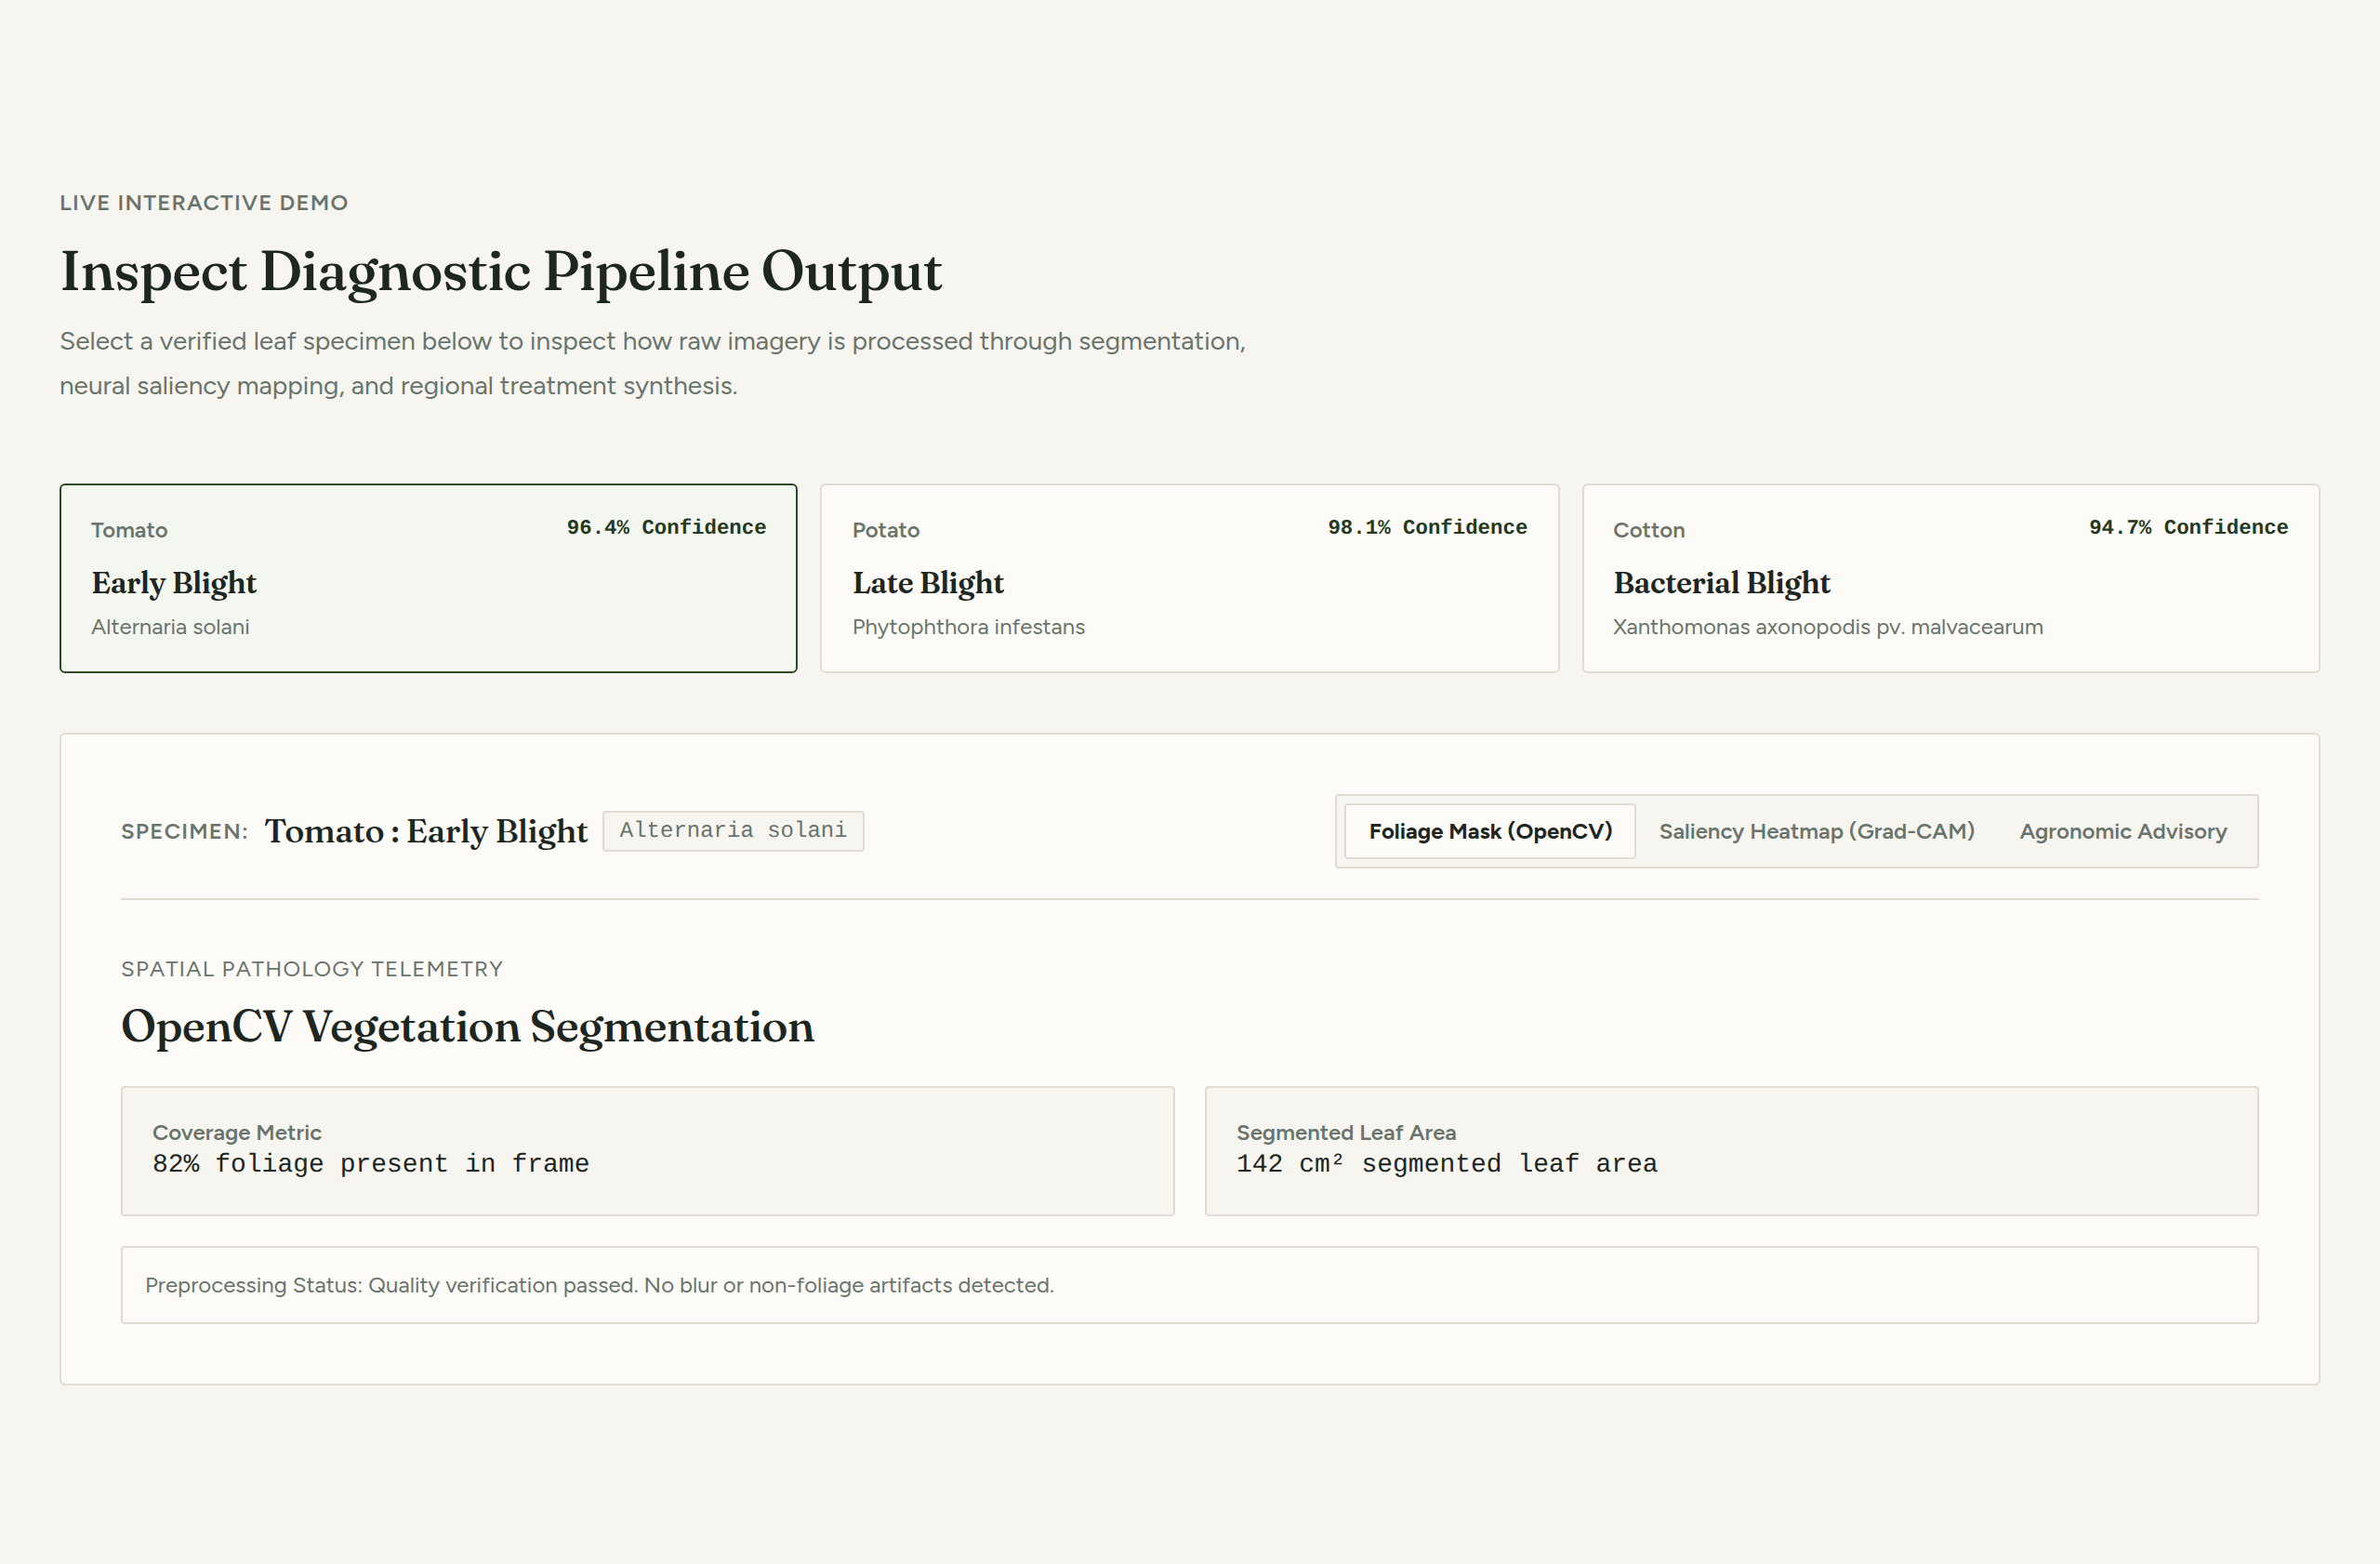
\includegraphics[width=\linewidth]{screenshots/08_demo_workbench_analysis.png}
  \caption*{(b) Preprocessing foliage segmentation and spatial leaf coverage telemetry.}
\end{minipage}\\[1.5ex]
\begin{minipage}{0.48\textwidth}
  \centering
  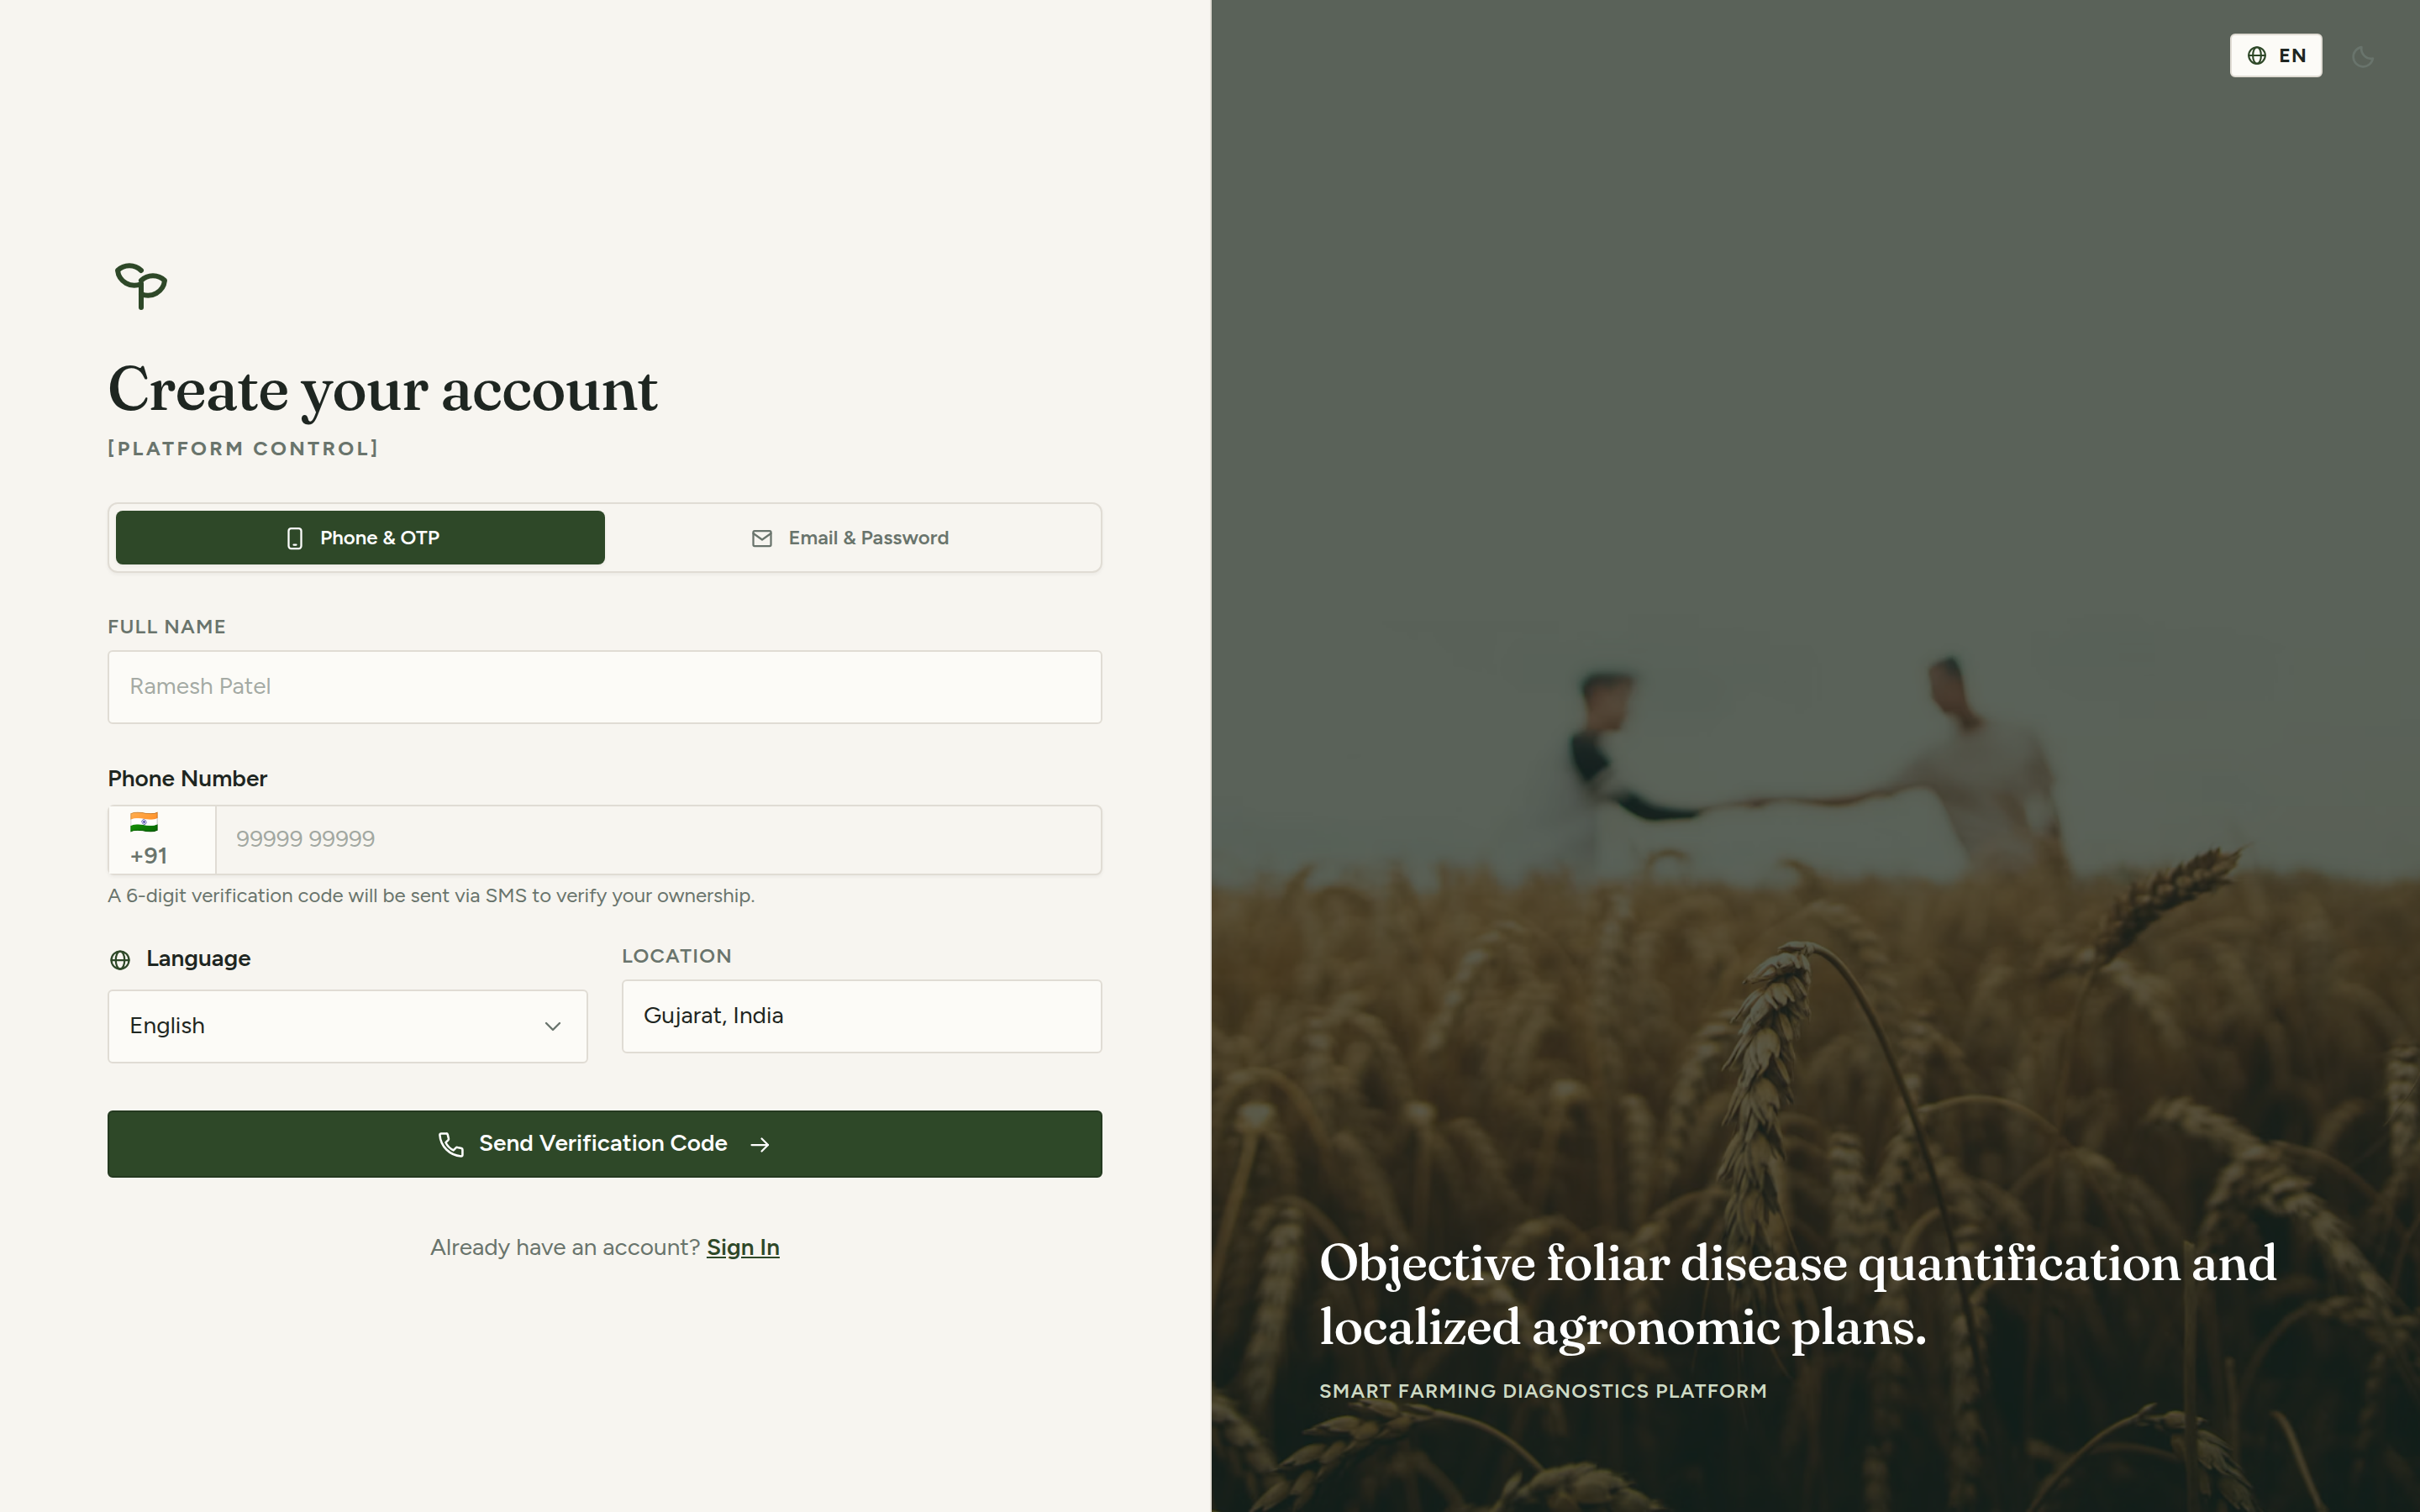
\includegraphics[width=\linewidth]{screenshots/06_register_page.png}
  \caption*{(c) Farmer onboarding with regional language selection.}
\end{minipage}\hfill
\begin{minipage}{0.48\textwidth}
  \centering
  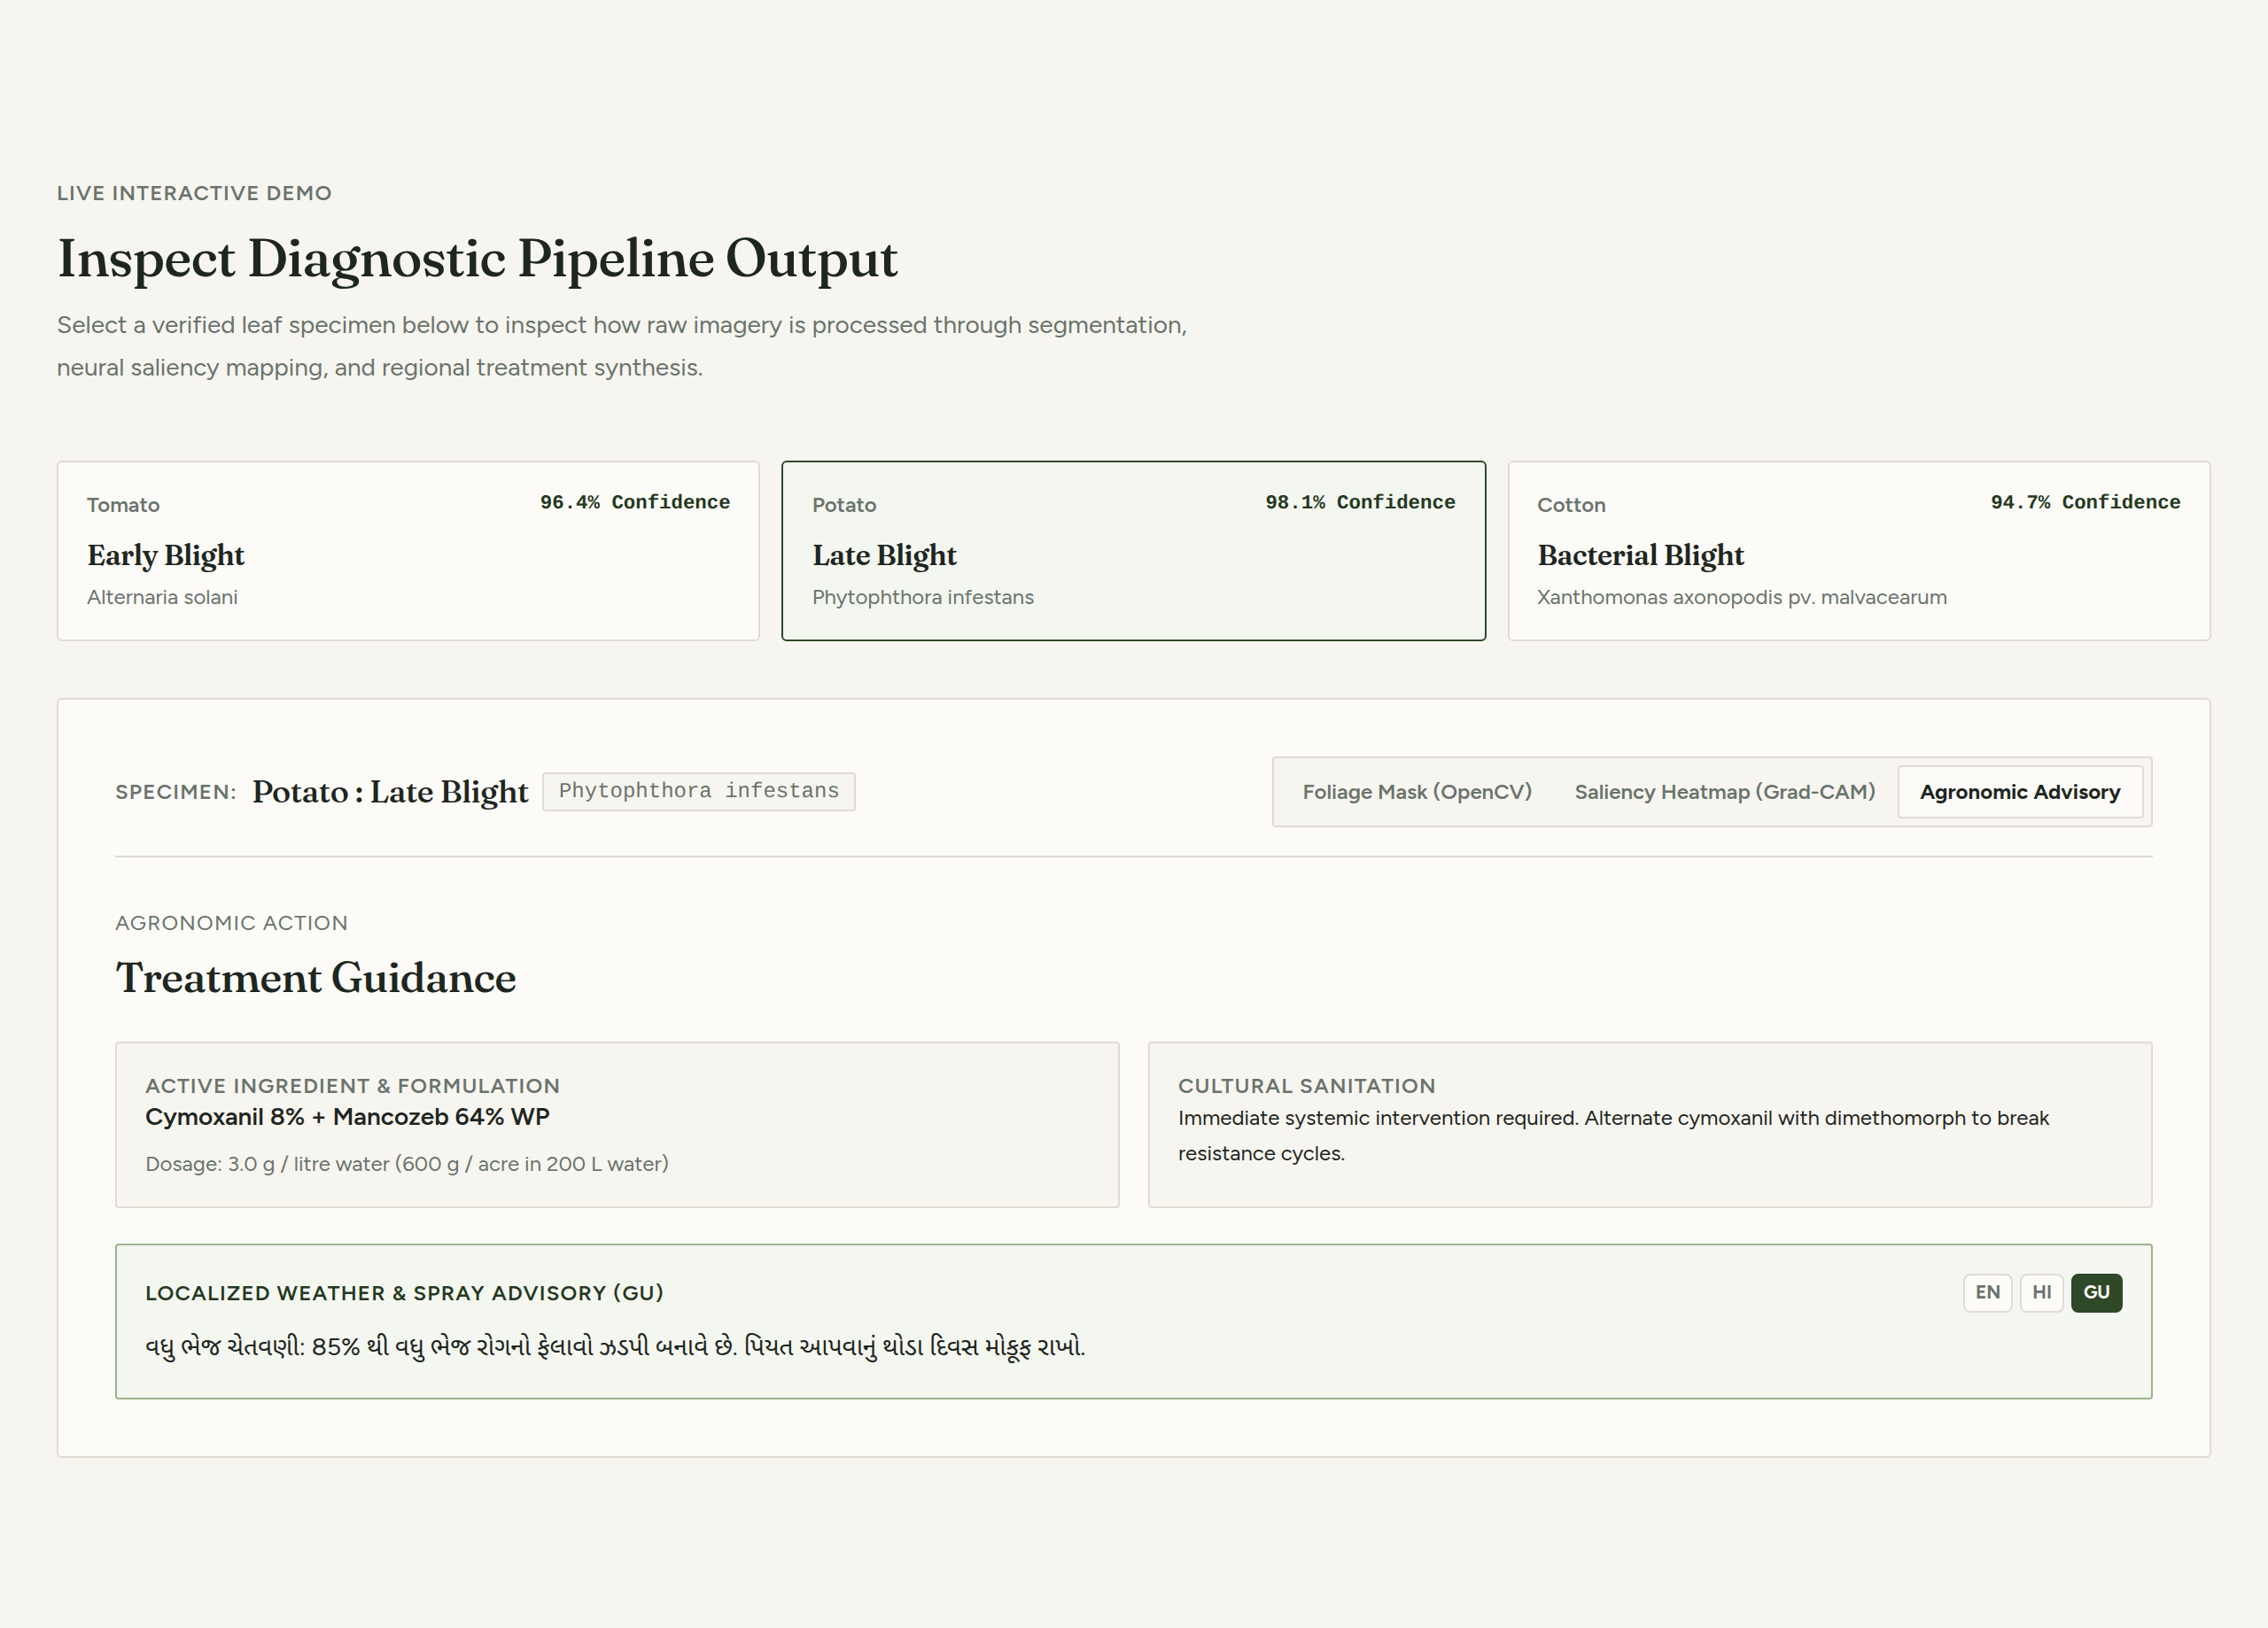
\includegraphics[width=\linewidth]{screenshots/12_demo_workbench_potato_late_blight.png}
  \caption*{(d) Severe disease classification and ICAR/KVK-grounded chemical formulation.}
\end{minipage}
\caption{Comprehensive platform interface gallery illustrating user onboarding, foliage quality gate segmentation, and disease classification with localized treatment dosage.}
\label{fig:platform-gallery}
\end{figure*}

\begin{table*}[!t]
\centering
\small
\caption{Platform Interface Demonstration and Verification Artifacts}
\label{tab:screenshot_evidence}
\begin{tabularx}{\textwidth}{l p{5.5cm} X}
\toprule
\textbf{No.} & \textbf{Screenshot} & \textbf{What it should demonstrate}\\
\midrule
1 & Landing page & Product identity and entry points.\\
2 & Registration/login & Authentication flow; use dummy account data.\\
3 & Image upload or camera screen & Supported file types and upload experience.\\
4 & Prediction result & Crop, disease, severity, confidence, and recommendation display.\\
5 & Prediction history & Past scans and status indicators.\\
6 & Plot/farm management & Farm details and plot association.\\
7 & Expert review queue & Cases awaiting review.\\
8 & Expert review detail & Image, model output, correction controls, and review action.\\
9 & Admin dashboard & Metrics or operational overview.\\
10 & Model registry / MLOps page & Training run and promotion workflow, if implemented.\\
11 & Language and audio controls & Gujarati/Hindi selection and narration, if available.\\
12 & Mobile home/result screens & Actual Flutter implementation and responsive workflow.\\
\bottomrule
\end{tabularx}
\end{table*}

\section{Reproducibility Checklist}
\begin{itemize}
\item Clone the open-source GitHub repository: \url{https://github.com/manthan2876/Smart-Farming}.
\item Verify the live web deployment at \url{https://smart-farming-dashboard-green.vercel.app}.
\item Open-source licensing and compliance: The complete source code and model pipeline configurations are licensed under the permissive \textbf{Apache License, Version 2.0} (see repository \texttt{LICENSE} and third-party attribution in \texttt{NOTICE}). No external registration or proprietary patent fee is required for educational and research evaluation.
\item Academic integrity and attribution: Foundational models and frameworks (PyTorch, Ultralytics YOLOv8, EfficientNet, IndicTrans2, Edge-TTS, FastAPI, React) are explicitly credited in compliance with university academic integrity standards.
\item Record the Git commit hash and date used to build the report.
\item Record the exact dataset export ID, timestamp, and manifest hash.
\item Record checkpoint hashes, model names, label-map hashes, and preprocessing version.
\item Record the deployed API URL and AI service revision; remove secrets from all screenshots.
\item Run unit, API, authorisation, integration, and end-to-end tests.
\item Attach actual model metrics rather than copying illustrative values.
\item Confirm all endpoint paths against the deployed OpenAPI schema.
\item Compile the LaTeX file and check references, figures, and table overflow.
\end{itemize}


\end{document}
